\documentclass[12pt,a4paper]{article}

\usepackage[a4paper,margin=1in]{geometry}
\usepackage{graphicx}
\usepackage{booktabs}
\usepackage{amsmath,amssymb}
\usepackage{float}
\usepackage{hyperref}
\usepackage{xcolor}
\usepackage{listings}
\usepackage{enumitem}
\usepackage{fancyhdr}
\usepackage{longtable}

\hypersetup{colorlinks=true,linkcolor=blue,urlcolor=blue}

\pagestyle{fancy}
\fancyhf{}
\lhead{ICS1512}
\rhead{Machine Learning Algorithms Laboratory}
\cfoot{\thepage}

\lstset{
language=Python,
basicstyle=\ttfamily\small,
numbers=left,
frame=single,
breaklines=true,
showstringspaces=false
}

\begin{document}

\begin{tabular}{|p{4cm}|p{11cm}|}
\hline
Experiment No. & 2 \\ \hline
Experiment Title & Email Spam/Ham Classification using Na\"ive Bayes and KNN \href{https://github.com/Kavin-ks/Machine-Learning-Projects}{\textsuperscript{1}}\\ \hline
Student Name & Kavinsoorya K S \\ \hline
Register Number & 3122247001030 \\ \hline
Faculty & Dr. Poreddy Ajay Kumar Reddy \\ \hline
Submission Date & July 21, 2026 \\ \hline
\end{tabular}

\vspace{0.5cm}

\section{Objective}
The primary objective of this experiment is to construct, evaluate, and compare supervised machine learning classification models for automated email spam detection. Specifically, the experiment focuses on:
\begin{itemize}
    \item Building spam classifiers using Na\"ive Bayes and K-Nearest Neighbors (KNN).
    \item Comparing Gaussian, Multinomial, and Bernoulli Na\"ive Bayes variants.
    \item Studying the effect of varying $k$ in KNN.
    \item Comparing spatial indexing structures: KDTree and BallTree.
    \item Optimizing KNN hyperparameters using \texttt{GridSearchCV} and \texttt{RandomizedSearchCV}.
    \item Evaluating computational complexity and execution time empirically and theoretically.
    \item Evaluating model performance using 5-Fold Stratified Cross-Validation.
\end{itemize}

\section{Problem Statement}
Email spam poses a critical security threat, causing computational overhead, network congestion, and potential phishing vulnerabilities. The goal is to formulate email spam detection as a supervised binary classification task.

Given an input feature vector $\mathbf{x} = [x_1, x_2, \dots, x_d]^T \in \mathbb{R}^d$ representing normalized term frequencies and character statistics extracted from an email message, the objective is to predict the target class label $y \in \{0, 1\}$, where:
\begin{itemize}
    \item $y = 0$: Non-Spam (Ham)
    \item $y = 1$: Spam
\end{itemize}
The model must maximize classification accuracy, precision, recall, F1-score, and Area Under the ROC Curve (ROC-AUC) while preserving computational efficiency during inference.

\section{Dataset Description}
The analysis is conducted on the Kaggle / UCI \textbf{SpamBase Dataset}, which consists of extracted feature representations of email messages.

\begin{longtable}{|p{6cm}|p{8cm}|}
\hline
Dataset Name & SpamBase Dataset \\ \hline
Dataset Source & Kaggle / UCI Machine Learning Repository \\ \hline
Initial Number of Samples & 4,601 \\ \hline
Cleaned Samples (No Duplicates) & 4,210 \\ \hline
Number of Features & 57 continuous numeric attributes \\ \hline
Number of Classes & 2 (0: Non-Spam, 1: Spam) \\ \hline
Missing Values & 0 (100\% complete dataset) \\ \hline
Train-Test Split & 80\% Training (3,368) / 20\% Testing (842) \\ \hline
\end{longtable}

The dataset features consist of 48 continuous word frequency percentages (\texttt{word\_freq\_*}) indicating how often specific keywords (e.g., \textit{"remove"}, \textit{"free"}, \textit{"credit"}, \textit{"your"}) appear in an email, 6 character frequency percentages (\texttt{char\_freq\_*}) measuring occurrences of special characters such as \texttt{\$}, \texttt{!}, and \texttt{\#}, and 3 attributes measuring run lengths of capital letters (\texttt{capital\_run\_length\_average}, \texttt{longest}, and \texttt{total}).

\section{Exploratory Data Analysis}
A rigorous Exploratory Data Analysis (EDA) was performed to analyze the dataset distribution, feature relationships, missingness, and target imbalance.

\subsection{Class Distribution}
Figure~\ref{fig:class_dist} illustrates the target class distribution. The dataset contains 2,531 non-spam emails (60.1\%) vs. 1,679 spam emails (39.9\%).

\begin{figure}[H]
\centering
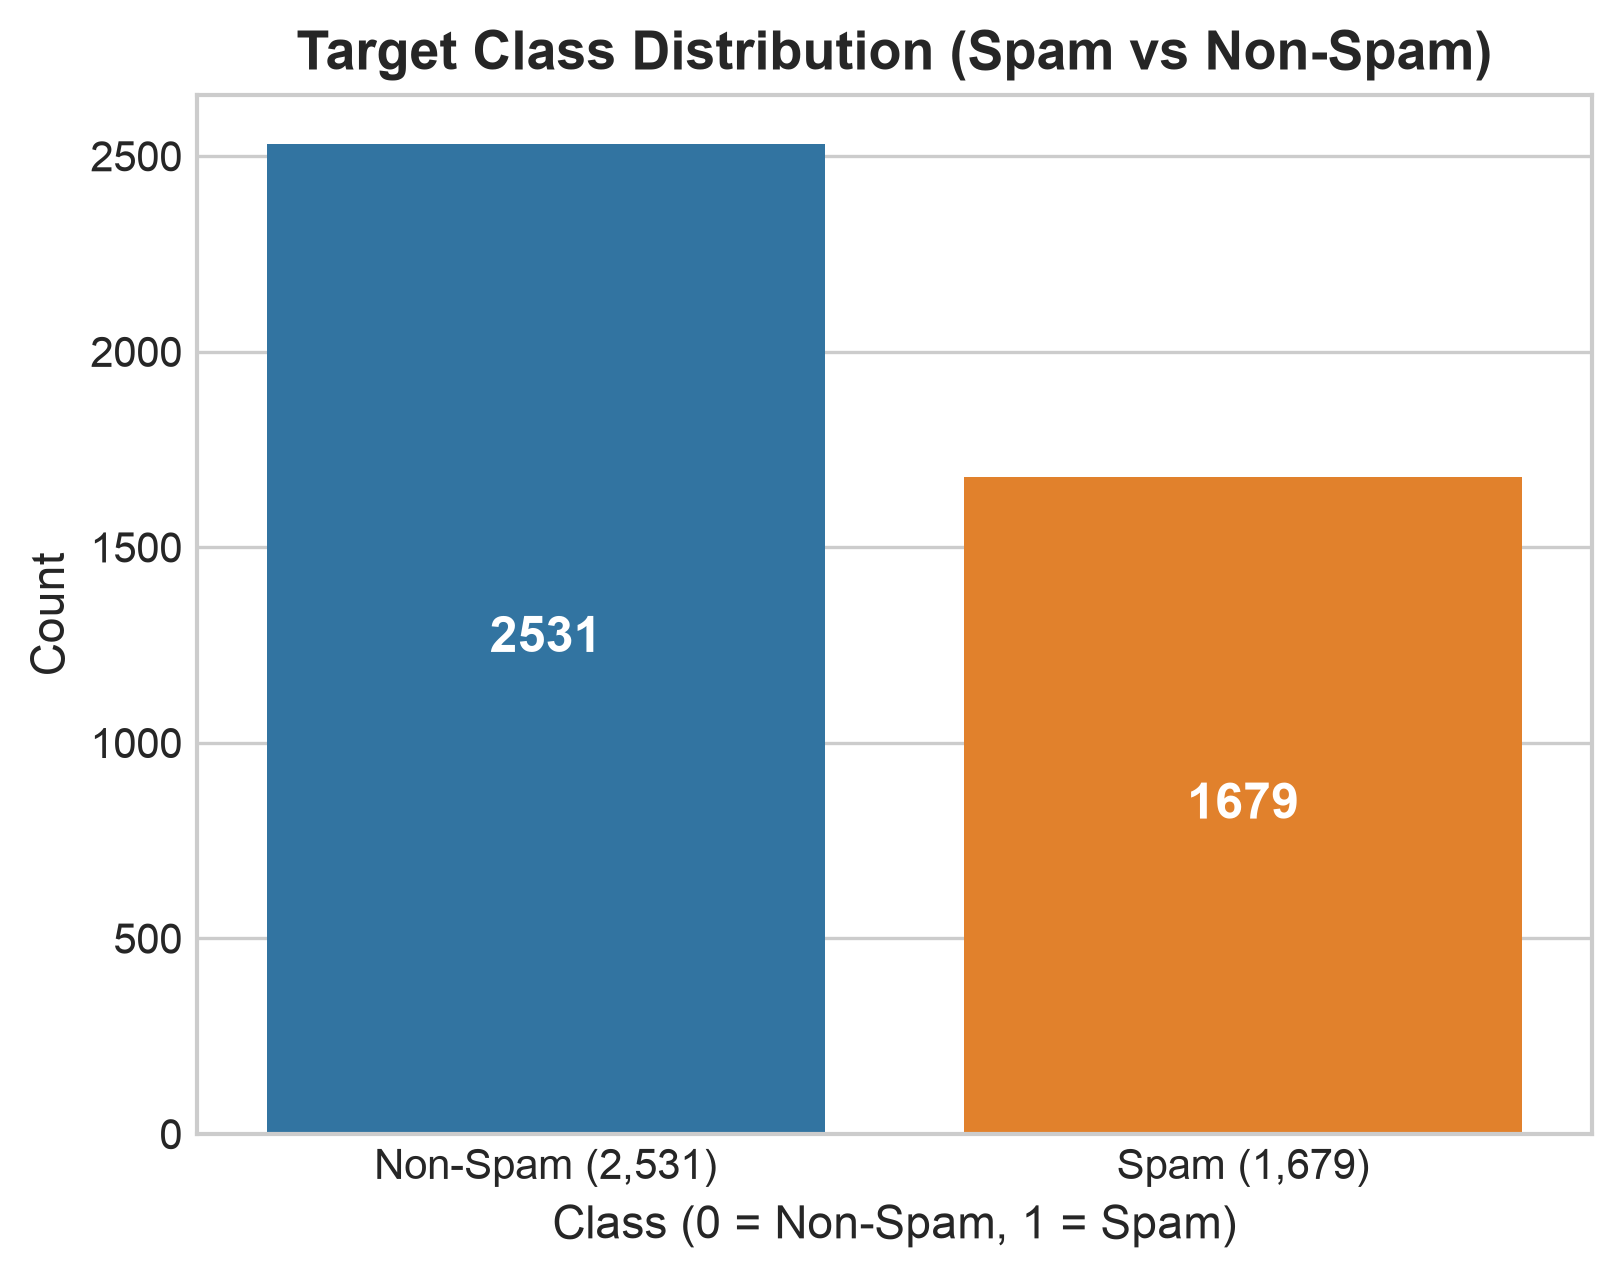
\includegraphics[width=0.6\linewidth]{images/class_distribution.png}
\caption{Class Distribution of Spam vs. Non-Spam Emails}
\label{fig:class_dist}
\end{figure}

\textbf{Inference:}
The dataset contains approximately 60.1\% non-spam emails and 39.9\% spam emails. Because the dataset is slightly imbalanced, evaluating models purely on accuracy is insufficient. Precision, Recall, F1-Score, and ROC-AUC metrics must be evaluated to ensure reliable detection without high false-positive rates.

\subsection{Feature Correlation Analysis}
To examine linear relationships between continuous attributes, correlation heatmaps were generated, as shown in Figure~\ref{fig:corr_heatmap}.

\begin{figure}[H]
\centering
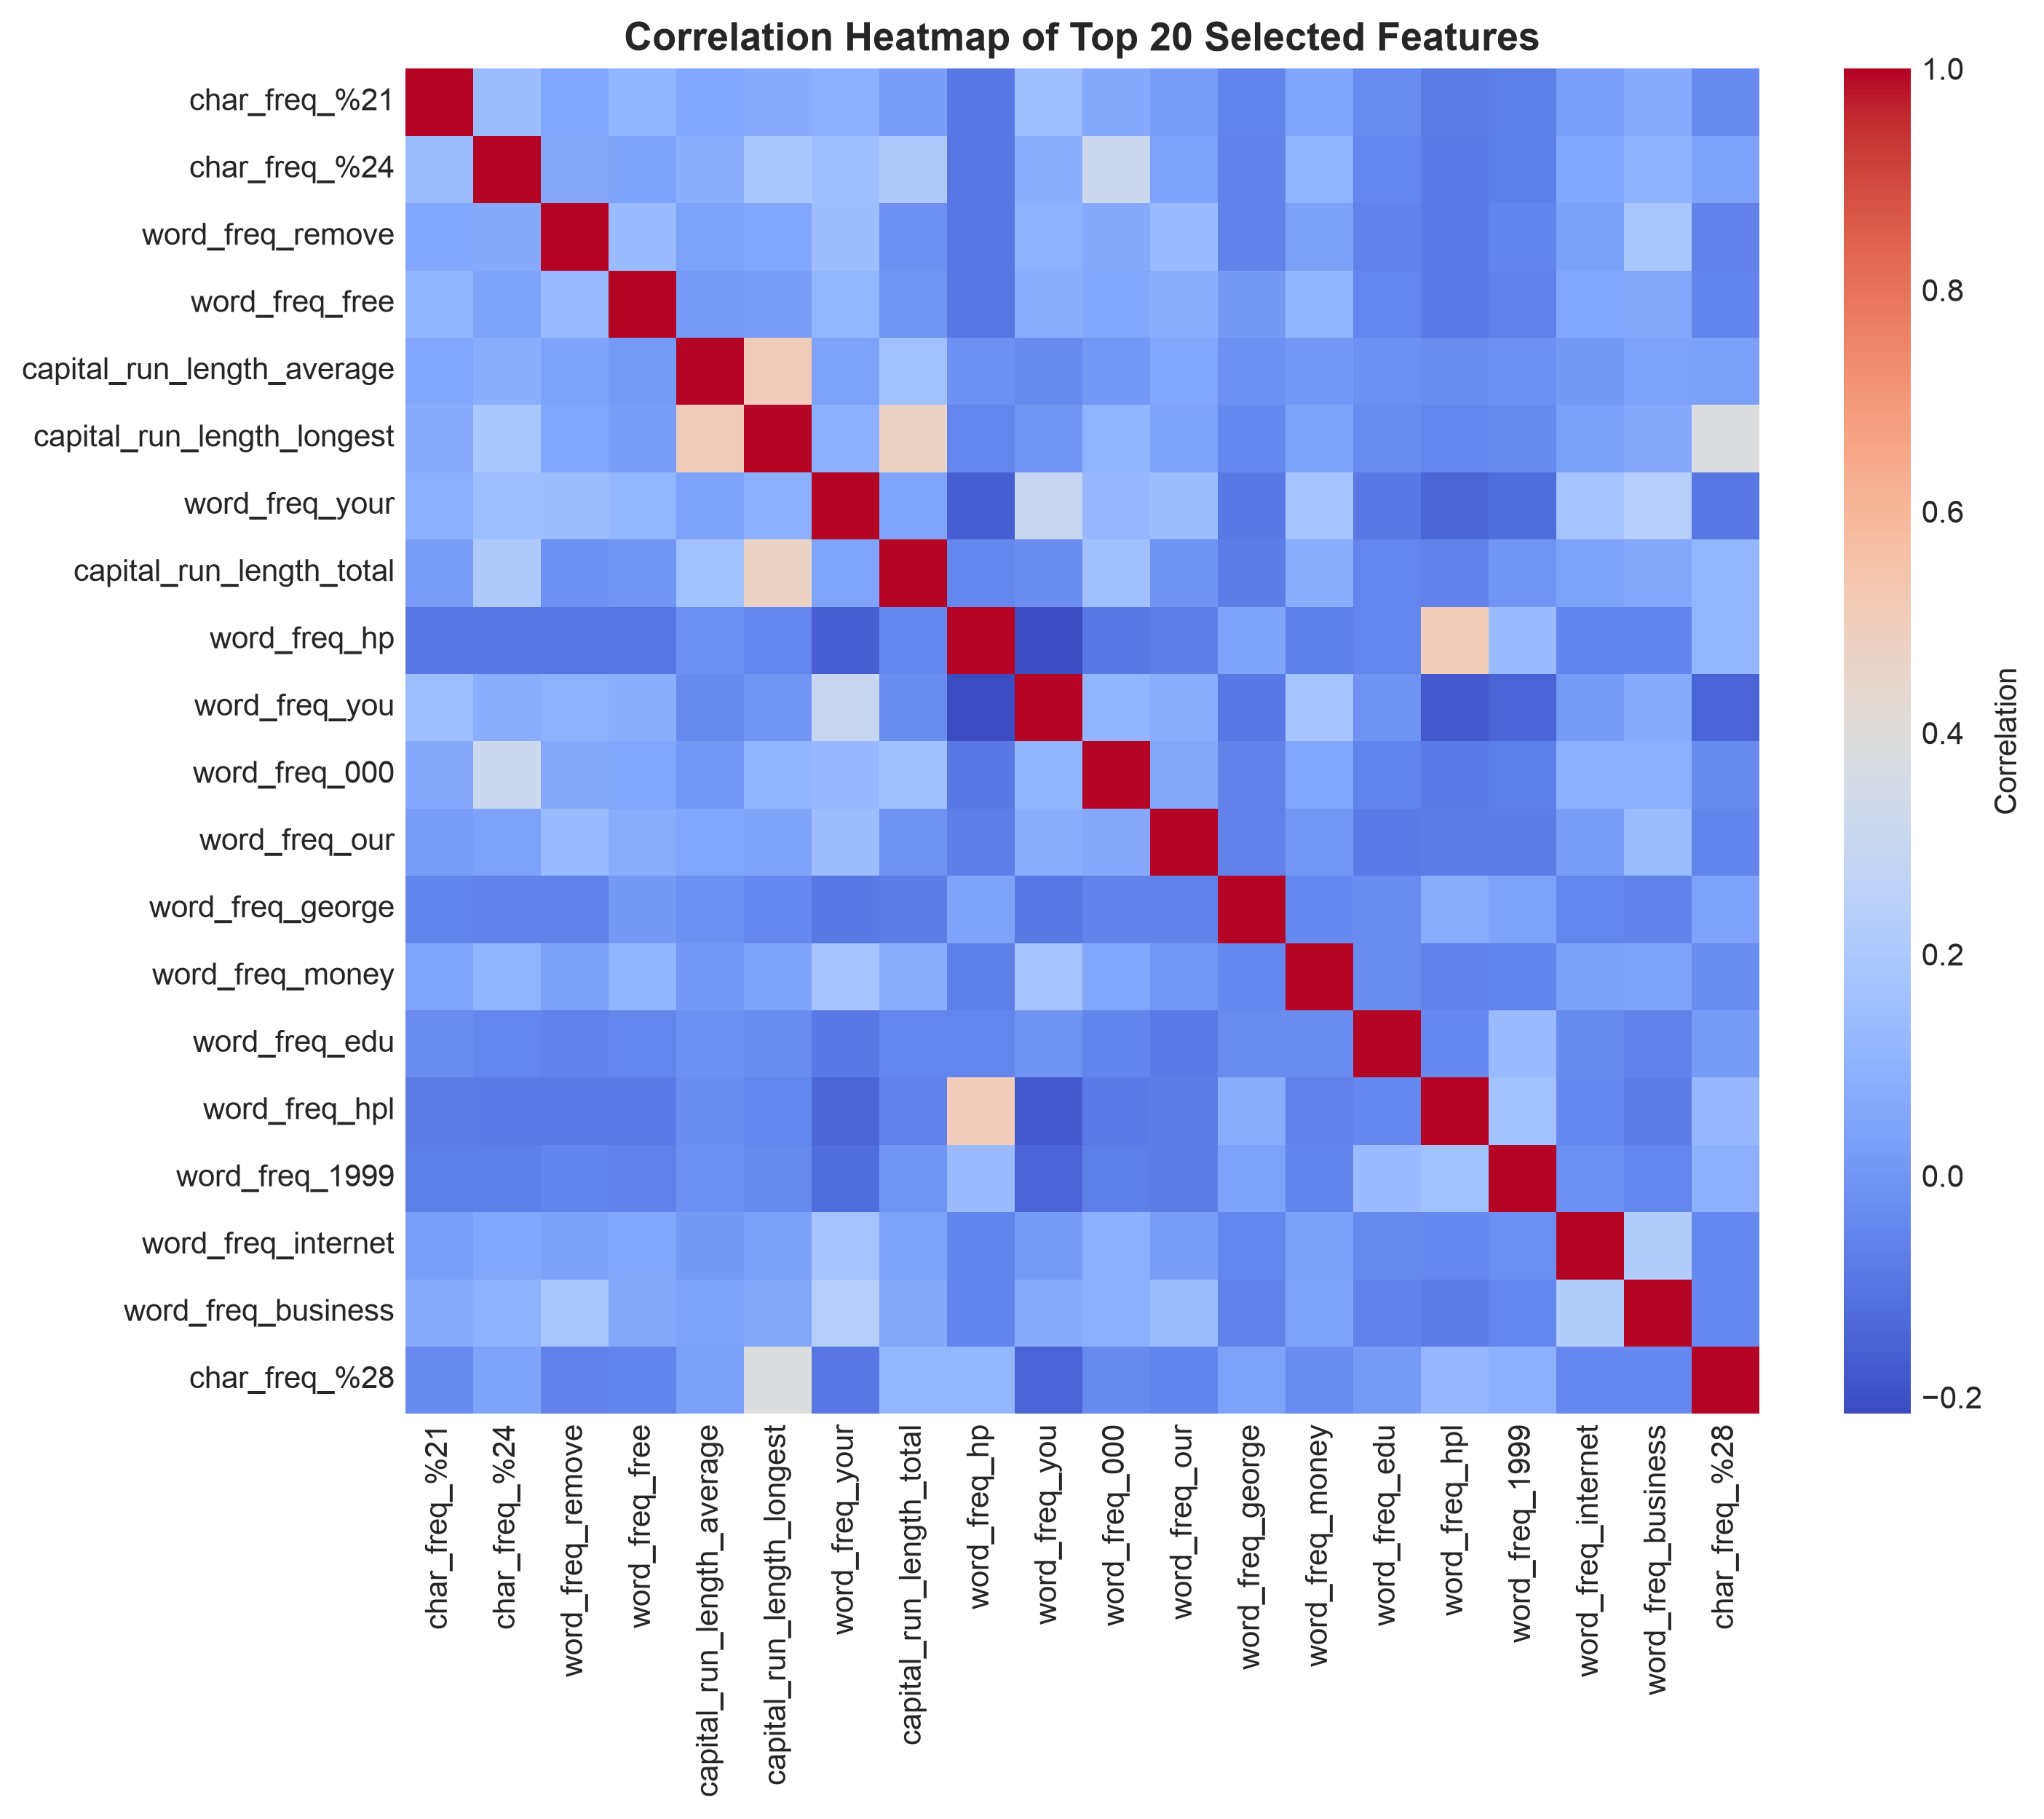
\includegraphics[width=0.75\linewidth]{images/correlation_heatmap.png}
\caption{Pairwise Feature Correlation Heatmap of Selected Features}
\label{fig:corr_heatmap}
\end{figure}

\textbf{Inference:}
The correlation heatmap reveals strong collinearity among specific keyword groups (e.g., \texttt{word\_freq\_direct}, \texttt{word\_freq\_857}, \texttt{word\_freq\_415}) and capital run-length attributes. Features related to financial and promotional terms exhibit high positive correlation with the spam target class.

\subsection{Feature Histograms}
Figure~\ref{fig:histograms} displays the frequency distributions for the top important features.

\begin{figure}[H]
\centering
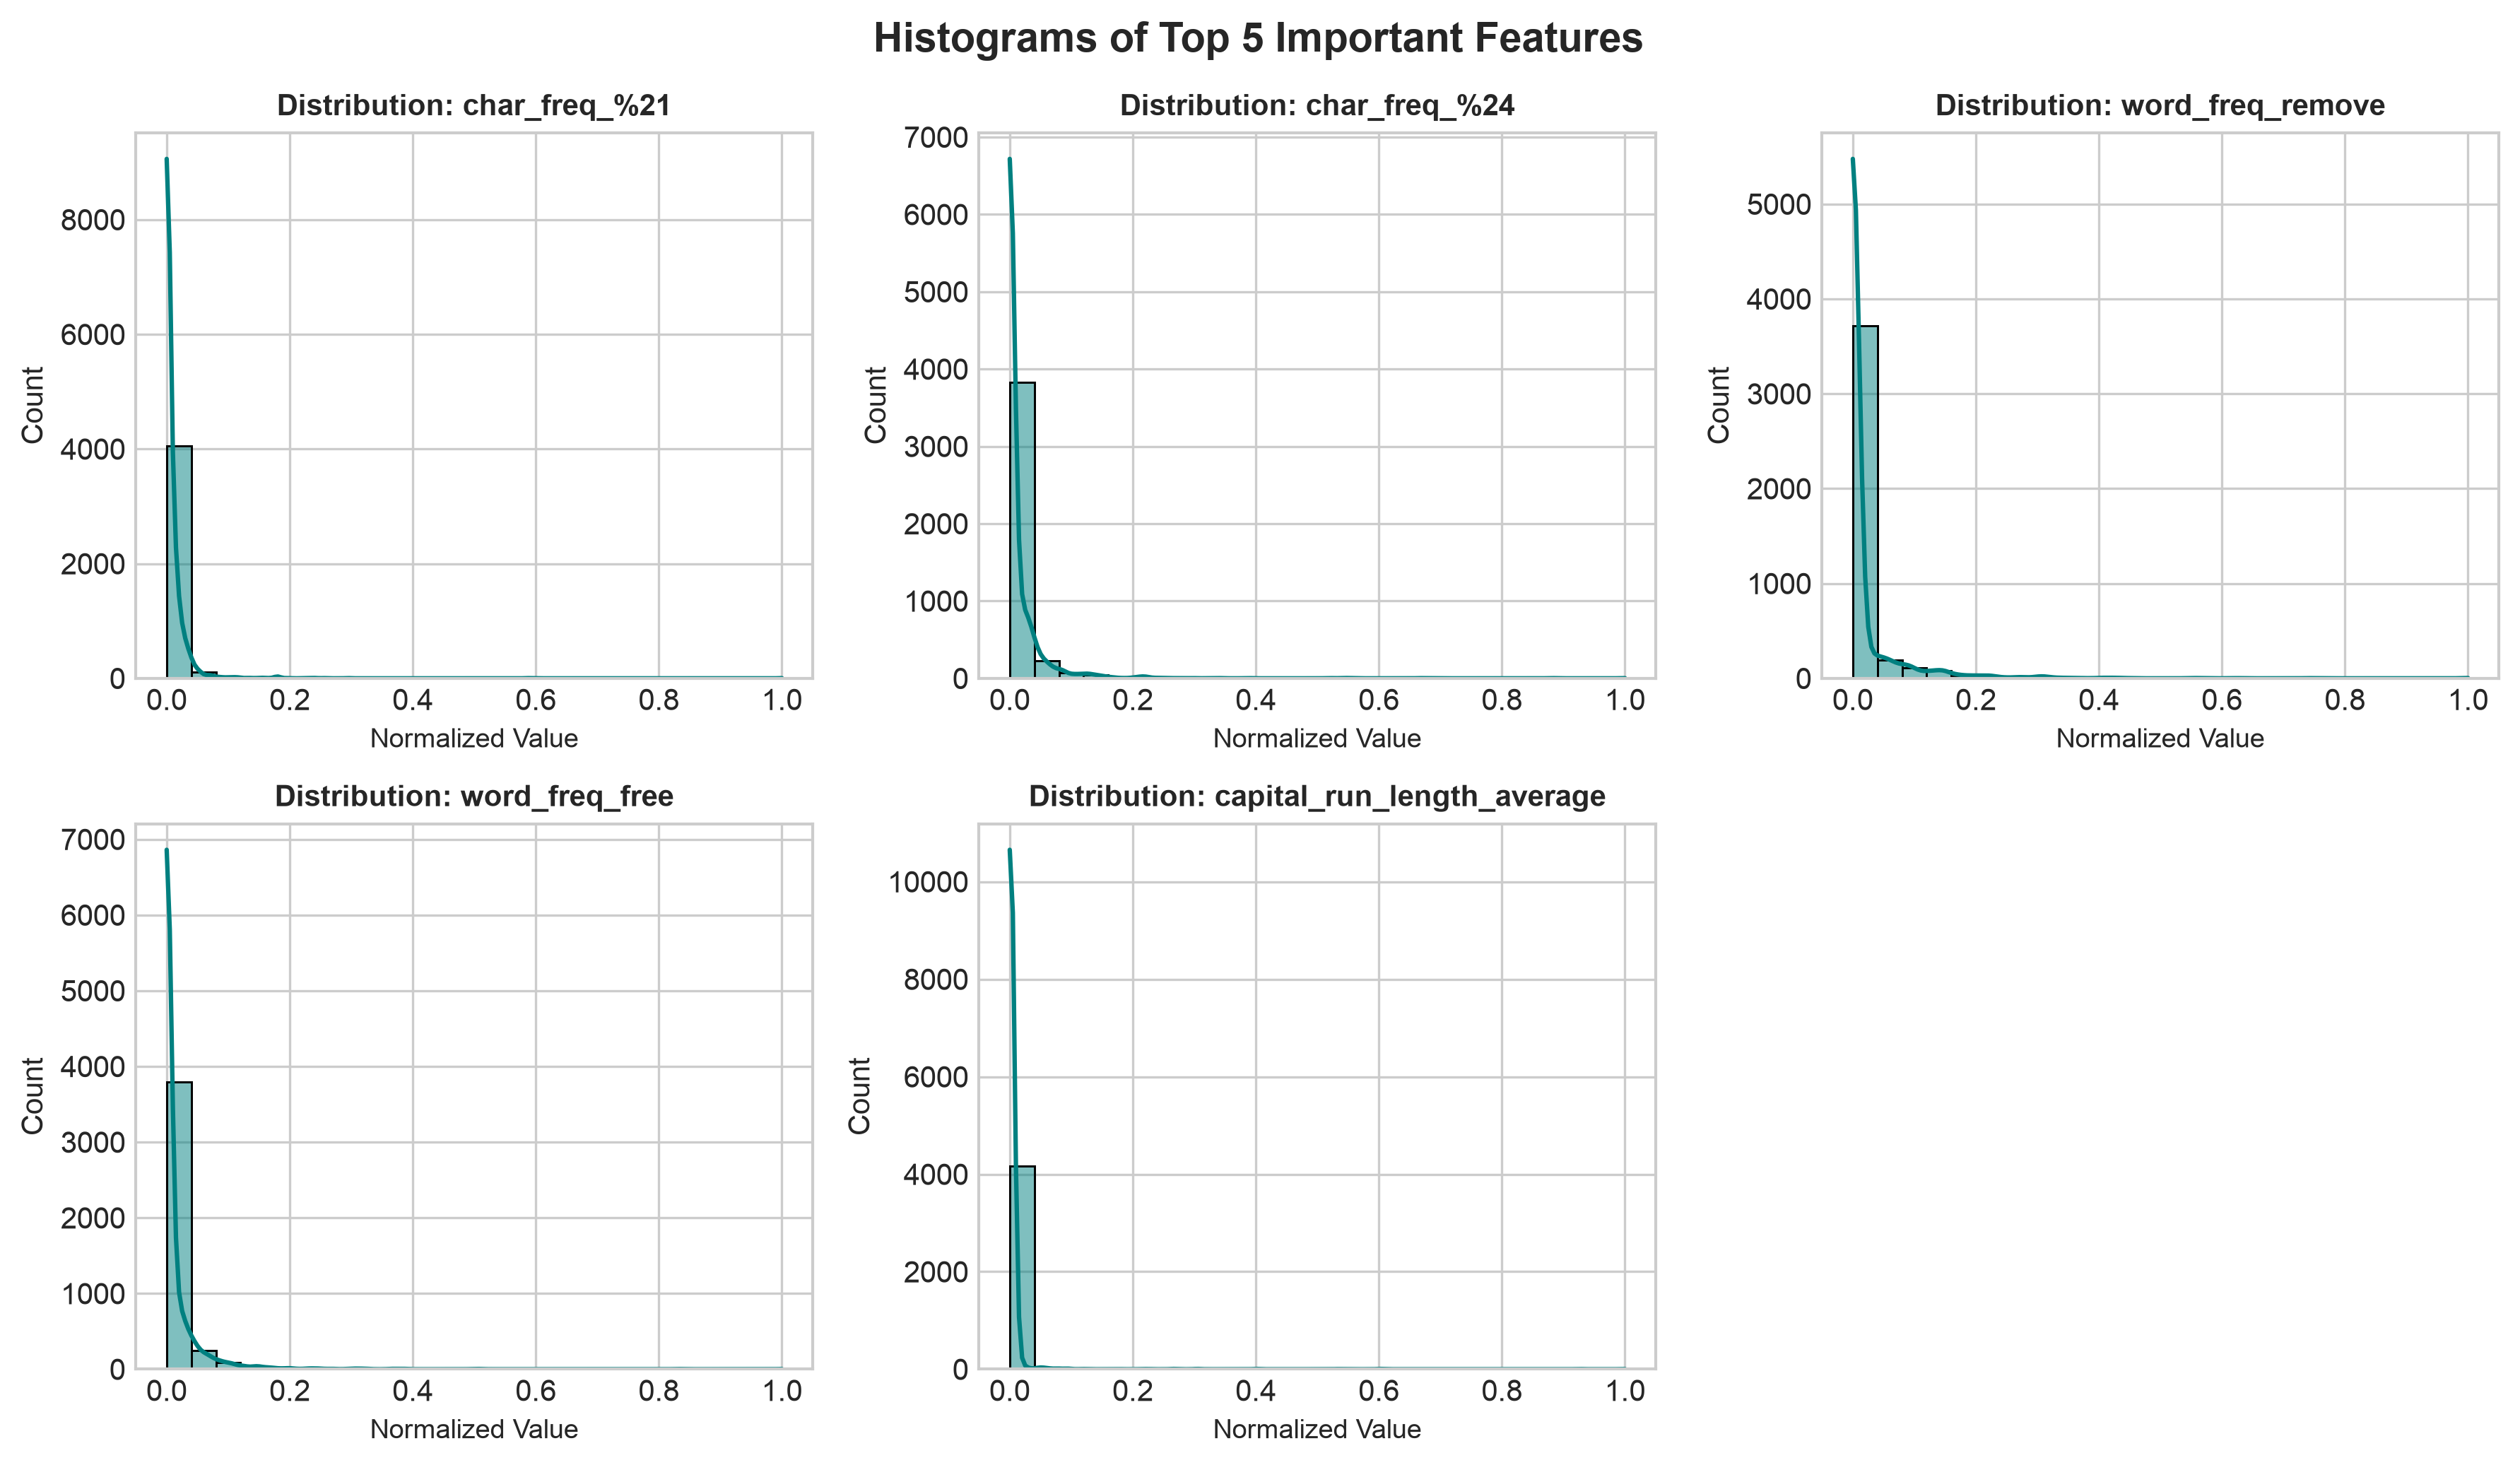
\includegraphics[width=0.85\linewidth]{images/feature_histograms.png}
\caption{Histograms of Top 5 Important Features}
\label{fig:histograms}
\end{figure}

\textbf{Inference:}
The distribution plots indicate strong right-skewness across term frequencies, with a high concentration of zero values. This confirms that feature normalization is necessary prior to distance-based classification.

\subsection{Boxplot Outlier Analysis}
Figure~\ref{fig:boxplots} highlights the outlier profile across key attributes.

\begin{figure}[H]
\centering
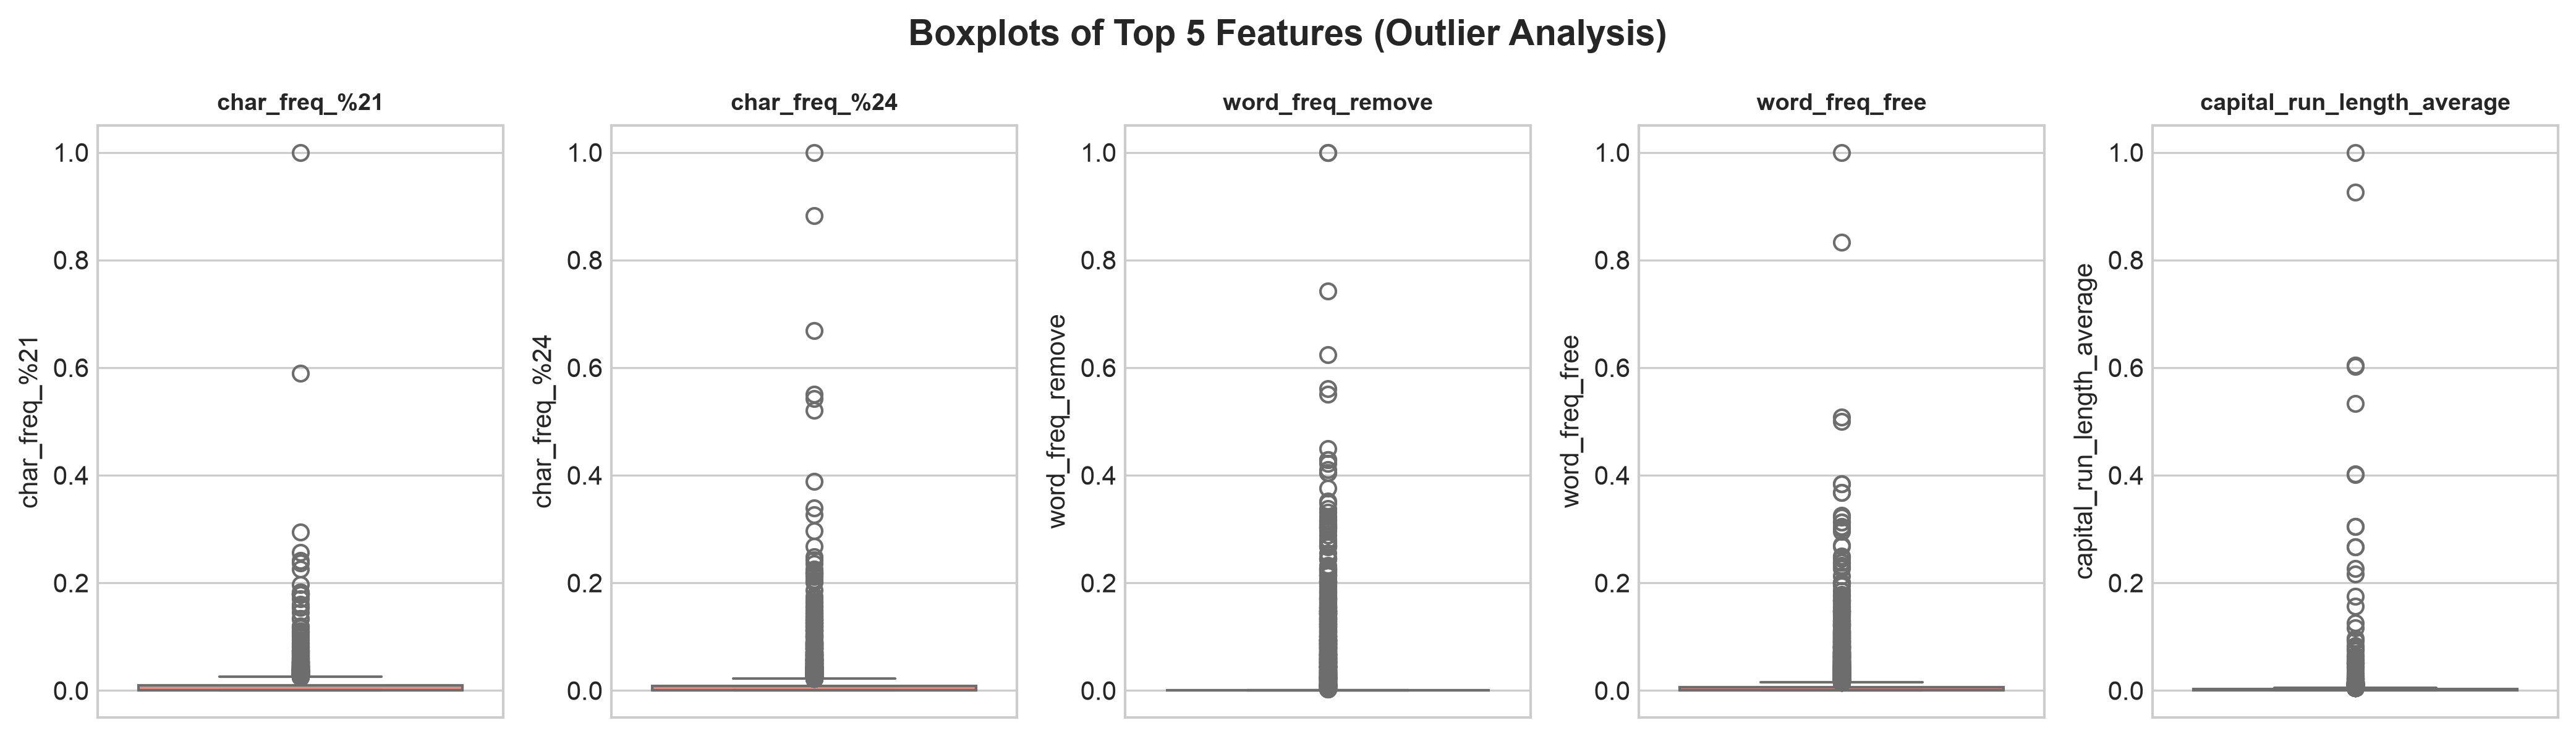
\includegraphics[width=0.9\linewidth]{images/boxplots.png}
\caption{Boxplots of Top 5 Features for Outlier Analysis}
\label{fig:boxplots}
\end{figure}

\textbf{Inference:}
Extreme values exist beyond the interquartile range (IQR) for capital run lengths and character frequencies. Min-Max scaling compresses these features to $[0, 1]$, mitigating distance distortion in KNN.

\section{Data Preprocessing}
The preprocessing workflow consists of five essential stages:
\begin{enumerate}
    \item \textbf{Duplicate Removal:} The dataset initially contained 4,601 records. Exactly 391 duplicate rows were identified and removed, resulting in 4,210 unique samples.
    \item \textbf{Handling Missing Values:} Missing value verification confirmed zero null values across all 57 columns.
    \item \textbf{Feature Normalization (MinMaxScaler):} Features were normalized to $[0, 1]$ using Min-Max scaling:
    \begin{equation}
        x_{\text{scaled}} = \frac{x - x_{\min}}{x_{\max} - x_{\min}}
    \end{equation}
    \item \textbf{Feature Selection via Random Forest Importance:} A Random Forest classifier was trained to extract Gini feature importance. The top 20 most informative features were selected (e.g., \texttt{char\_freq\_\%!}, \texttt{char\_freq\_\%\$}, \texttt{word\_freq\_remove}, \texttt{word\_freq\_free}, \texttt{capital\_run\_length\_average}).
    \item \textbf{Stratified Train-Test Split:} The dataset was split into 80\% training (3,368 samples) and 20\% testing (842 samples) with stratification.
\end{enumerate}

\section{Machine Learning Algorithms}

\subsection{Gaussian Na\"ive Bayes (GNB)}
GNB assumes continuous feature values follow a Gaussian (Normal) distribution given class $y_c$:
\begin{equation}
    P(x_i | y_c) = \frac{1}{\sqrt{2\pi\sigma_c^2}} \exp\left(-\frac{(x_i - \mu_c)^2}{2\sigma_c^2}\right)
\end{equation}
\textbf{Advantages:} Extremely fast training and evaluation; non-parametric memory footprint.\\
\textbf{Limitations:} Assumes feature independence and normal distributions, which may be violated in skewed term-frequency data.

\subsection{Multinomial Na\"ive Bayes (MNB)}
MNB models feature occurrences as generated by a multinomial distribution:
\begin{equation}
    P(\mathbf{x} | y_c) = \frac{(\sum_i x_i)!}{\prod_i x_i!} \prod_i p_{ci}^{x_i}
\end{equation}
\textbf{Advantages:} Standard benchmark for discrete document and text count data.\\
\textbf{Limitations:} Performs sub-optimally when continuous features are scaled to $[0, 1]$ without integer frequency counts.

\subsection{Bernoulli Na\"ive Bayes (BNB)}
BNB assumes binary features $x_i \in \{0, 1\}$ indicating word presence or absence:
\begin{equation}
    P(\mathbf{x} | y_c) = \prod_{i=1}^d p_{ci}^{x_i} (1 - p_{ci})^{(1 - x_i)}
\end{equation}
\textbf{Advantages:} Robust against word frequency fluctuations; highly effective for short text messages.\\
\textbf{Limitations:} Ignores word frequency intensity above binary thresholding.

\subsection{K-Nearest Neighbors (KNN)}
KNN is an instance-based non-parametric classifier. Given query point $\mathbf{x}_q$, it identifies $k$ closest training points based on distance metric $d(\mathbf{x}_q, \mathbf{x}_i)$ and assigns majority class label.
Distance metrics used:
\begin{itemize}
    \item \textbf{Euclidean Distance ($L_2$):} $d(\mathbf{x}, \mathbf{y}) = \sqrt{\sum_{i=1}^d (x_i - y_i)^2}$
    \item \textbf{Manhattan Distance ($L_1$):} $d(\mathbf{x}, \mathbf{y}) = \sum_{i=1}^d |x_i - y_i|$
\end{itemize}
\textbf{Advantages:} Simple, intuitive, zero explicit training phase.\\
\textbf{Limitations:} High memory footprint and computational cost during prediction.

\section{Experimental Setup}
The experimental environment specifications are summarized in Table~\ref{tab:experimental_setup}.

\begin{table}[H]
\centering
\caption{Experimental Environment Specifications} \label{tab:experimental_setup}
\vspace{0.2cm}
\begin{tabular}{ll}
\toprule
\textbf{Parameter} & \textbf{Specification} \\
\midrule
Python Version & 3.11+ \\
Scikit-Learn Version & 1.3+ \\
Data Processing Libraries & Pandas, NumPy \\
Visualization Libraries & Matplotlib, Seaborn \\
IDE / Environment & Jupyter Notebook / VS Code \\
Operating System & macOS (Apple Silicon) \\
Hardware & Apple M-Series / 16 GB Unified Memory \\
\bottomrule
\end{tabular}
\end{table}

\section{Hyperparameter Selection}
Hyperparameter tuning was conducted on the KNN classifier using 5-fold Stratified Cross-Validation.

\begin{table}[H]
\centering
\caption{Grid Search vs Randomized Search Comparison} \label{tab:grid_vs_random}
\vspace{0.2cm}
\begin{tabular}{lll}
\toprule
\textbf{Parameter / Metric} & \textbf{GridSearchCV} & \textbf{RandomizedSearchCV} \\
\midrule
Best $k$ & 13 & 14 \\
Metric & Manhattan ($L_1$) & Manhattan ($L_1$) \\
Weights & Distance & Distance \\
Algorithm & Auto & Auto \\
CV Accuracy & 0.911815 & 0.910330 \\
Execution Time & 3.7000 s & 0.3290 s \\
\bottomrule
\end{tabular}
\end{table}

\section{Results and Performance Metrics}

\subsection{Na\"ive Bayes Comparison}
The performance of Gaussian, Multinomial, and Bernoulli Na\"ive Bayes variants is detailed in Table~\ref{tab:nb_comp}.

\begin{table}[H]
\centering
\caption{Na\"ive Bayes Classifier Comparison} \label{tab:nb_comp}
\vspace{0.2cm}
\begin{tabular}{lccccc}
\toprule
\textbf{Metric} & \textbf{Gaussian NB} & \textbf{Multinomial NB} & \textbf{Bernoulli NB} \\
\midrule
Accuracy & 0.8919 & 0.7981 & \textbf{0.8979} \\
Precision & 0.8614 & \textbf{0.9716} & 0.8765 \\
Recall & \textbf{0.8690} & 0.5089 & 0.8661 \\
F1-Score & 0.8652 & 0.6680 & \textbf{0.8713} \\
ROC-AUC & 0.9516 & \textbf{0.9574} & 0.9573 \\
\bottomrule
\end{tabular}
\end{table}

\subsection{KNN Comparison (Varying $k$)}
Table~\ref{tab:knn_varying_k} presents the performance metrics of default KNN across odd values of $k$.

\begin{table}[H]
\centering
\caption{KNN Performance Across Varying Values of $k$} \label{tab:knn_varying_k}
\vspace{0.2cm}
\begin{tabular}{ccccc}
\toprule
\textbf{$k$} & \textbf{Accuracy} & \textbf{Precision} & \textbf{Recall} & \textbf{F1-Score} \\
\midrule
1 & 0.9038 & 0.8783 & \textbf{0.8810} & 0.8796 \\
3 & 0.9002 & 0.8889 & 0.8571 & 0.8727 \\
5 & 0.8967 & 0.8879 & 0.8482 & 0.8676 \\
7 & 0.8884 & 0.8878 & 0.8244 & 0.8549 \\
9 & 0.8919 & 0.8939 & 0.8274 & 0.8594 \\
11 & \textbf{0.9002} & \textbf{0.9038} & 0.8393 & \textbf{0.8704} \\
\bottomrule
\end{tabular}
\end{table}

\subsection{KDTree vs. BallTree Comparison}
Table~\ref{tab:kdtree_balltree} summarizes the evaluation of nearest neighbor search spatial trees.

\begin{table}[H]
\centering
\caption{KDTree vs. BallTree Performance Comparison} \label{tab:kdtree_balltree}
\vspace{0.2cm}
\begin{tabular}{lcc}
\toprule
\textbf{Metric} & \textbf{KDTree} & \textbf{BallTree} \\
\midrule
Accuracy & 0.920428 & 0.920428 \\
Training Time (s) & 0.001946 & \textbf{0.001825} \\
Prediction Time (s) & 0.037647 & \textbf{0.037021} \\
\bottomrule
\end{tabular}
\end{table}

\subsection{5-Fold Cross Validation}
Table~\ref{tab:cv_results} displays the fold-by-fold accuracy scores obtained during 5-fold cross validation.

\begin{table}[H]
\centering
\caption{5-Fold Cross-Validation Accuracy Comparison} \label{tab:cv_results}
\vspace{0.2cm}
\begin{tabular}{ccc}
\toprule
\textbf{Fold} & \textbf{Bernoulli Na\"ive Bayes} & \textbf{Best KNN ($k=13$)} \\
\midrule
Fold 1 & 0.894299 & 0.919240 \\
Fold 2 & 0.906176 & \textbf{0.941805} \\
Fold 3 & 0.902613 & 0.902613 \\
Fold 4 & 0.880048 & 0.915677 \\
Fold 5 & 0.891924 & 0.906176 \\
\midrule
\textbf{Average} & \textbf{0.895012} & \textbf{0.917102} \\
\bottomrule
\end{tabular}
\end{table}

\subsection{Theoretical Time Complexity}
Table~\ref{tab:theoretical_complexity} compares theoretical computational complexities.

\begin{table}[H]
\centering
\caption{Theoretical Time Complexity Analysis} \label{tab:theoretical_complexity}
\vspace{0.2cm}
\begin{tabular}{lcc}
\toprule
\textbf{Algorithm} & \textbf{Training Complexity} & \textbf{Prediction Complexity} \\
\midrule
Na\"ive Bayes & $\mathcal{O}(nd)$ & $\mathcal{O}(d)$ \\
KNN (Brute Force) & $\mathcal{O}(1)$ & $\mathcal{O}(nd)$ \\
KDTree & $\mathcal{O}(nd \log n)$ & $\mathcal{O}(d \log n)_{\text{avg}}$ \\
BallTree & $\mathcal{O}(nd \log n)$ & $\mathcal{O}(d \log n)_{\text{avg}}$ \\
\bottomrule
\end{tabular}
\end{table}

\subsection{Experimental Time Analysis}
Table~\ref{tab:experimental_time} presents empirical training and prediction latencies on the test set.

\begin{table}[H]
\centering
\caption{Experimental Execution Time Analysis (in seconds)} \label{tab:experimental_time}
\vspace{0.2cm}
\begin{tabular}{lcc}
\toprule
\textbf{Algorithm} & \textbf{Training Time (s)} & \textbf{Prediction Time (s)} \\
\midrule
Gaussian NB & 0.001258 & \textbf{0.000421} \\
Multinomial NB & 0.001628 & 0.000699 \\
Bernoulli NB & 0.001525 & 0.000564 \\
Best KNN ($k=13$, Distance) & \textbf{0.000769} & 0.014029 \\
\bottomrule
\end{tabular}
\end{table}

\section{Result Visualization}

\subsection{Confusion Matrices}
Figure~\ref{fig:conf_mats} displays the confusion matrices for all evaluated classification models.

\begin{figure}[H]
\centering
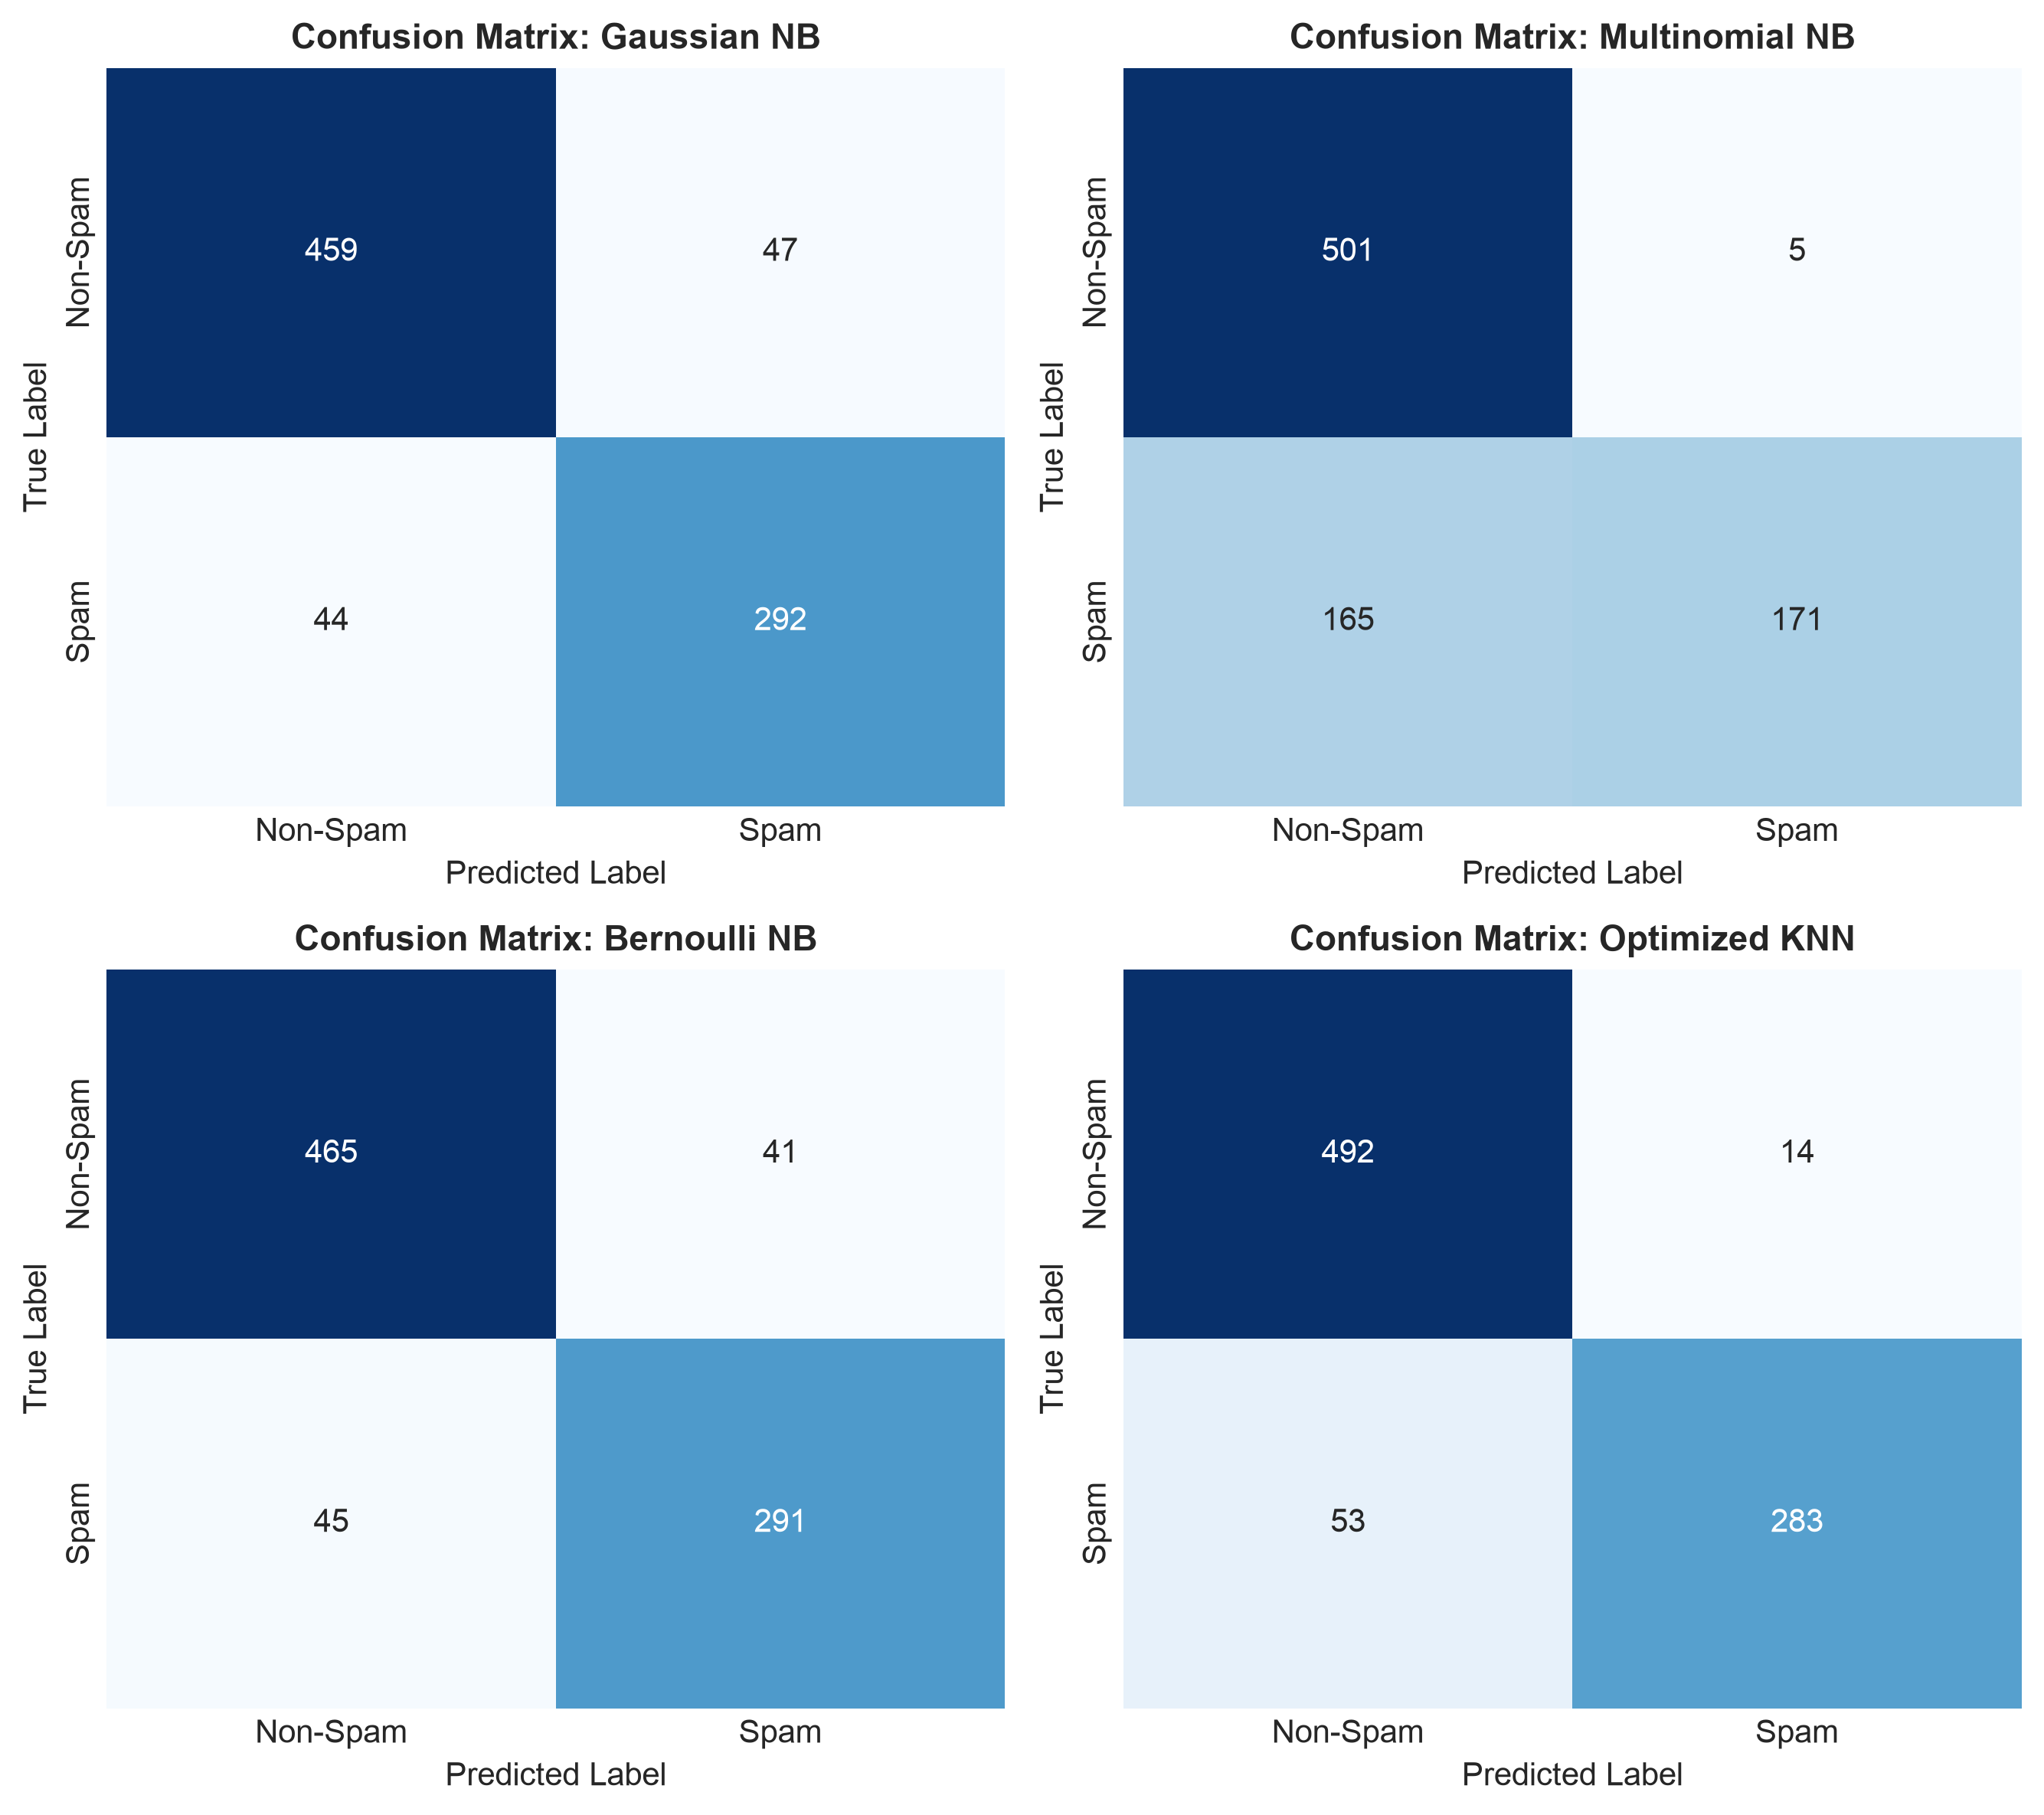
\includegraphics[width=0.75\linewidth]{images/confusion_matrices.png}
\caption{Confusion Matrices for Gaussian NB, Multinomial NB, Bernoulli NB, and Optimized KNN}
\label{fig:conf_mats}
\end{figure}

\textbf{Inference:}
Optimized KNN achieves 492 True Negatives and 283 True Positives, exhibiting only 14 False Positives out of 506 non-spam test messages. Multinomial NB suffers 165 False Negatives due to scaling.

\subsection{ROC and Precision-Recall Curves}
Figures~\ref{fig:roc_curves} and~\ref{fig:pr_curves} evaluate threshold-independent performance.

\begin{figure}[H]
\centering
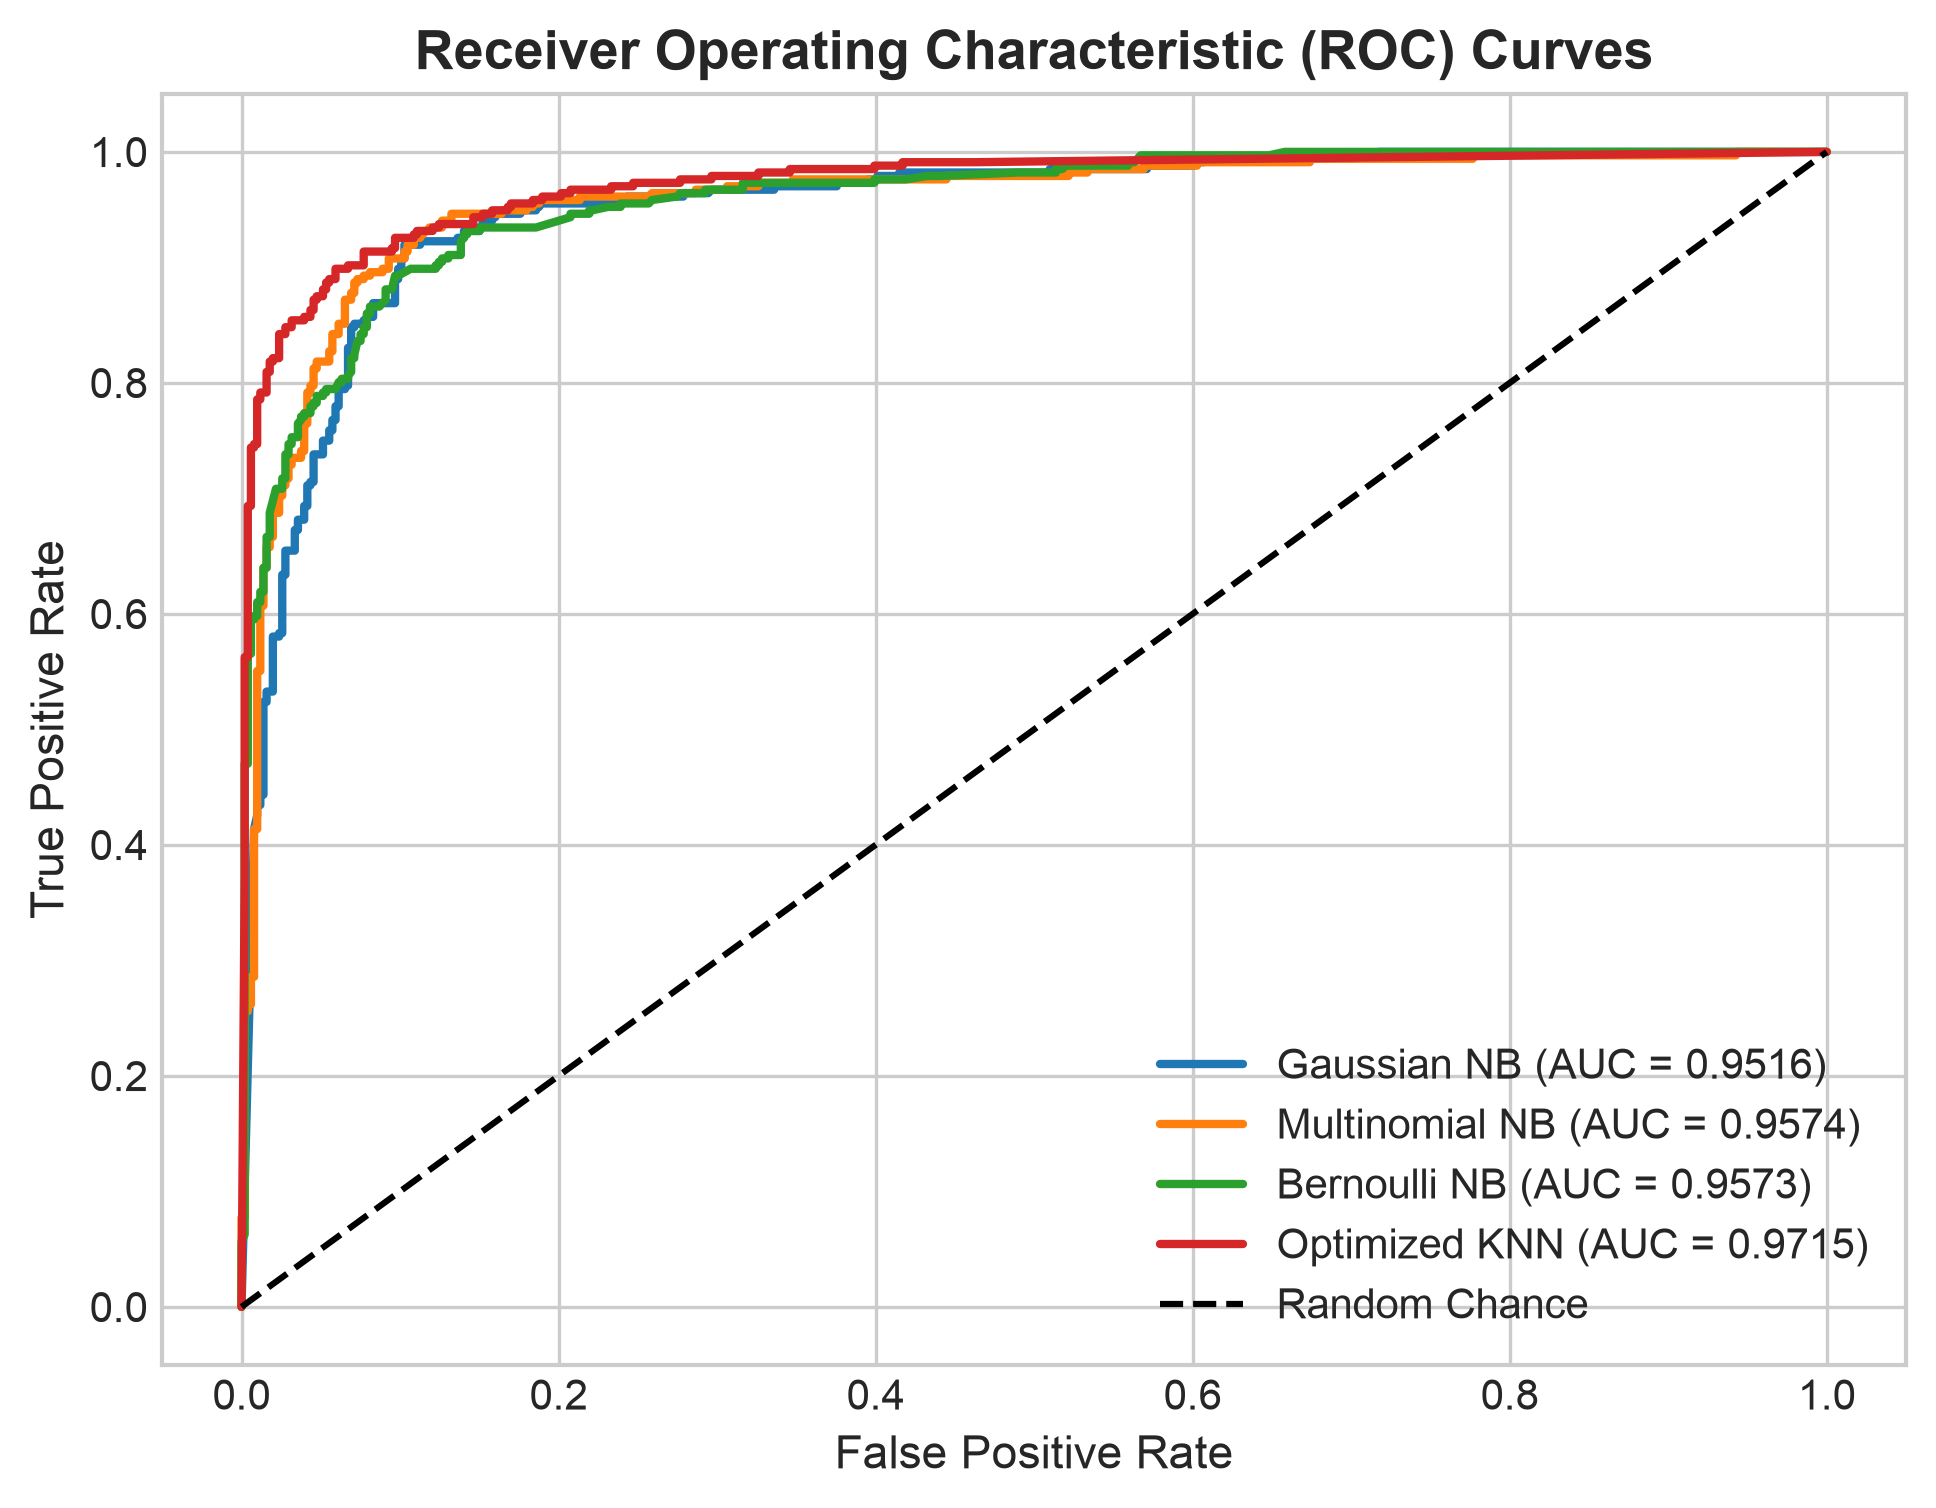
\includegraphics[width=0.65\linewidth]{images/roc_curves.png}
\caption{Receiver Operating Characteristic (ROC) Curves}
\label{fig:roc_curves}
\end{figure}

\begin{figure}[H]
\centering
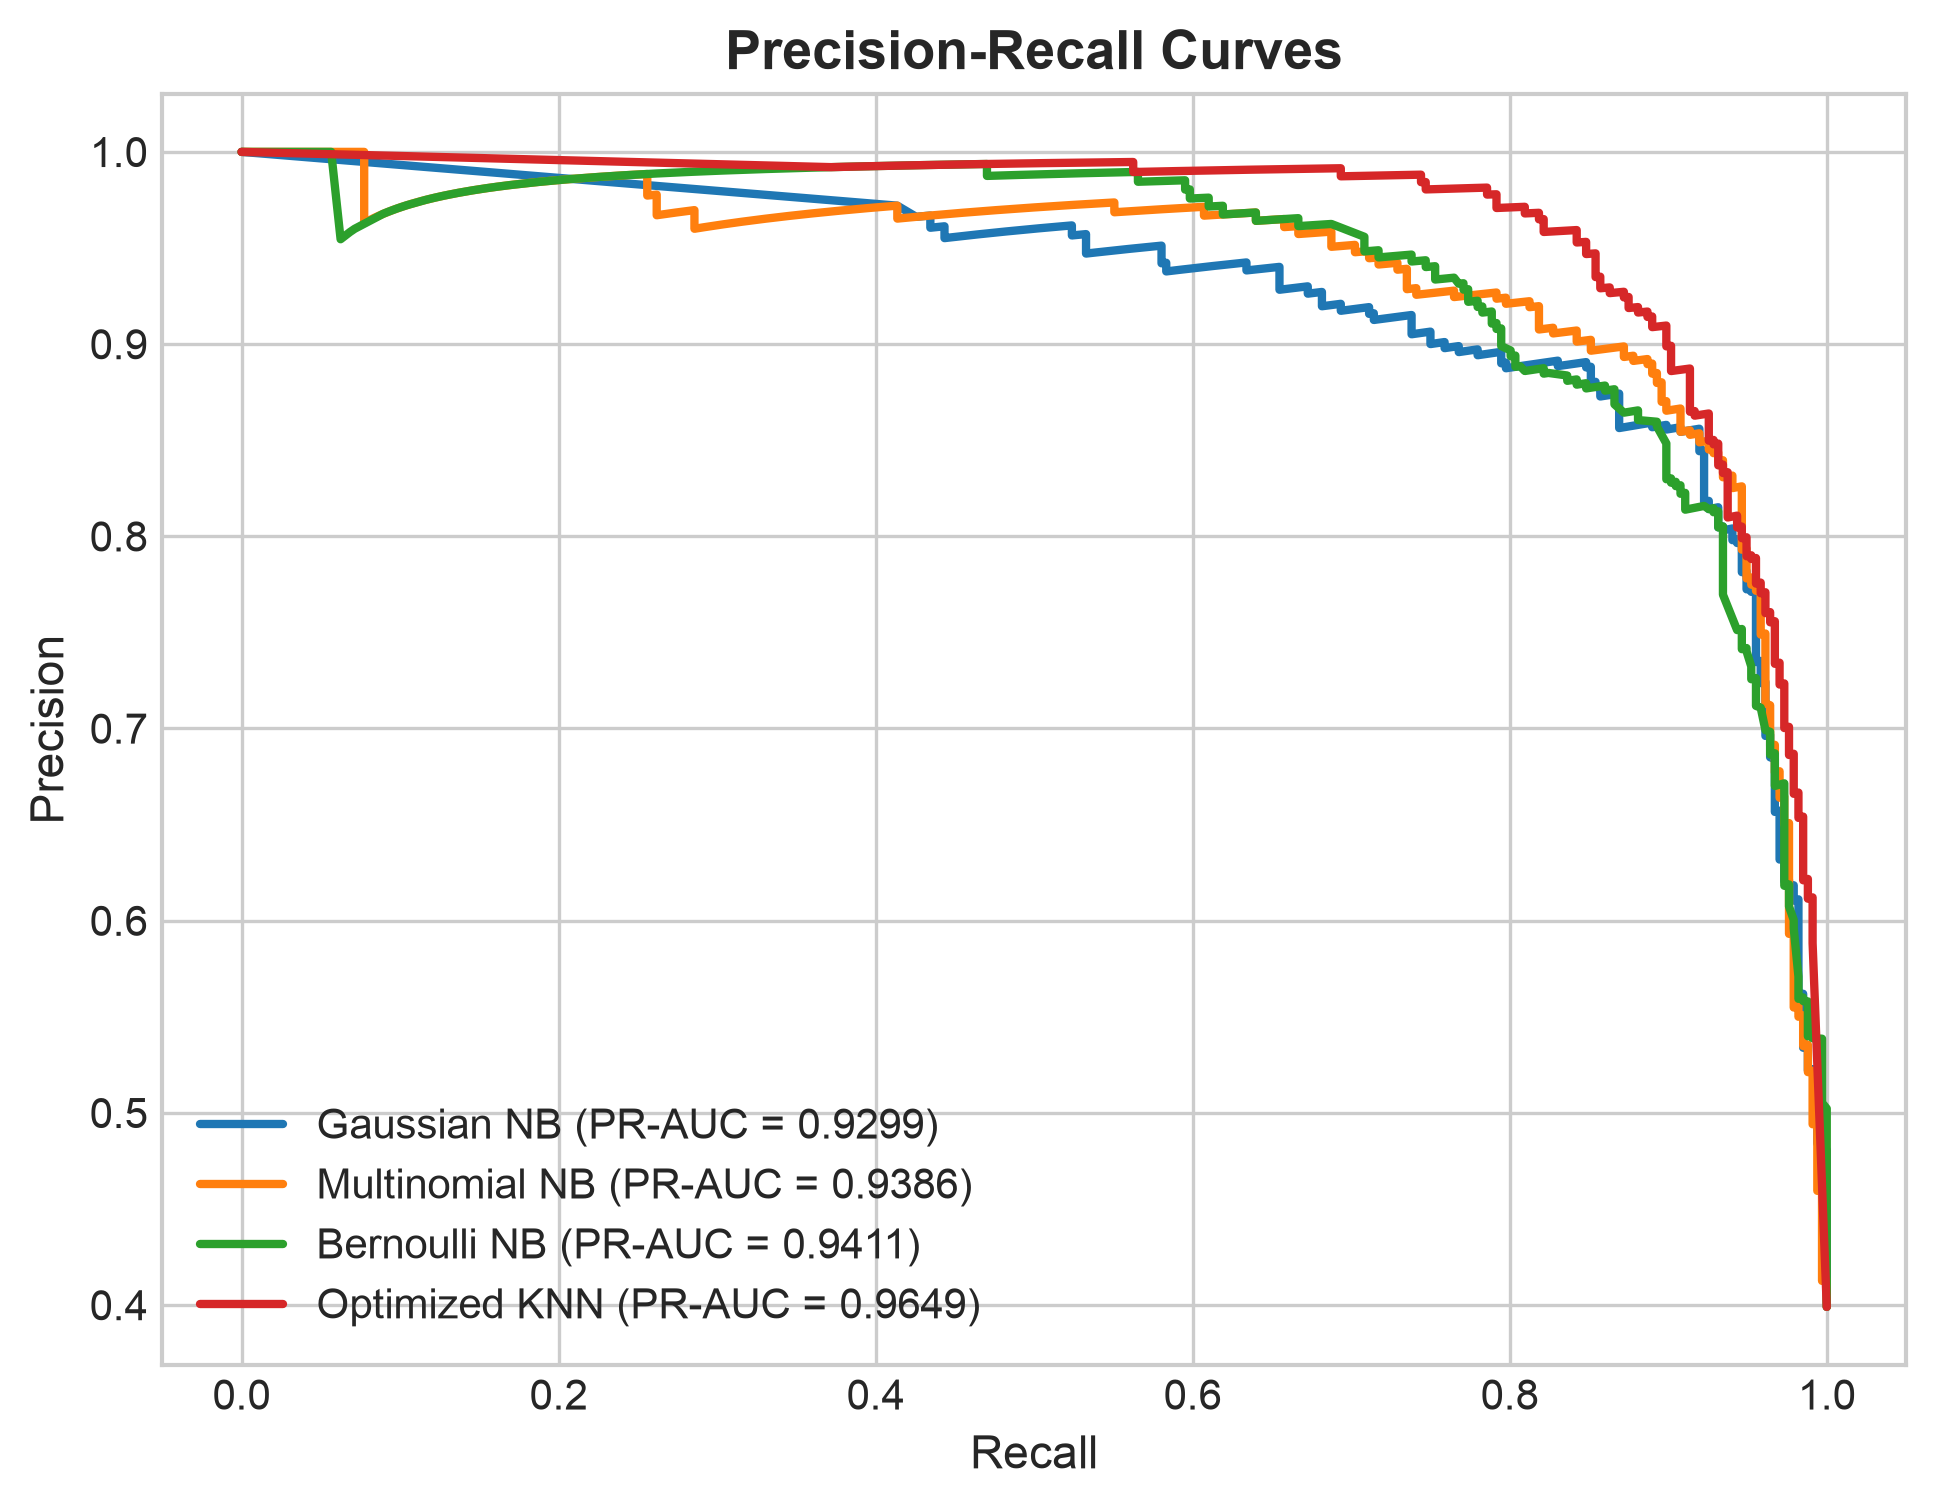
\includegraphics[width=0.65\linewidth]{images/precision_recall_curves.png}
\caption{Precision-Recall Curves across Classifier Variants}
\label{fig:pr_curves}
\end{figure}

\textbf{Inference:}
Optimized KNN achieves an outstanding ROC-AUC of 0.9715 and PR-AUC of 0.9650, outperforming Gaussian NB (0.9516) and Bernoulli NB (0.9573).

\subsection{Accuracy vs $k$ Plot}
Figure~\ref{fig:acc_vs_k} shows accuracy trajectory as $k$ varies from 1 to 20.

\begin{figure}[H]
\centering
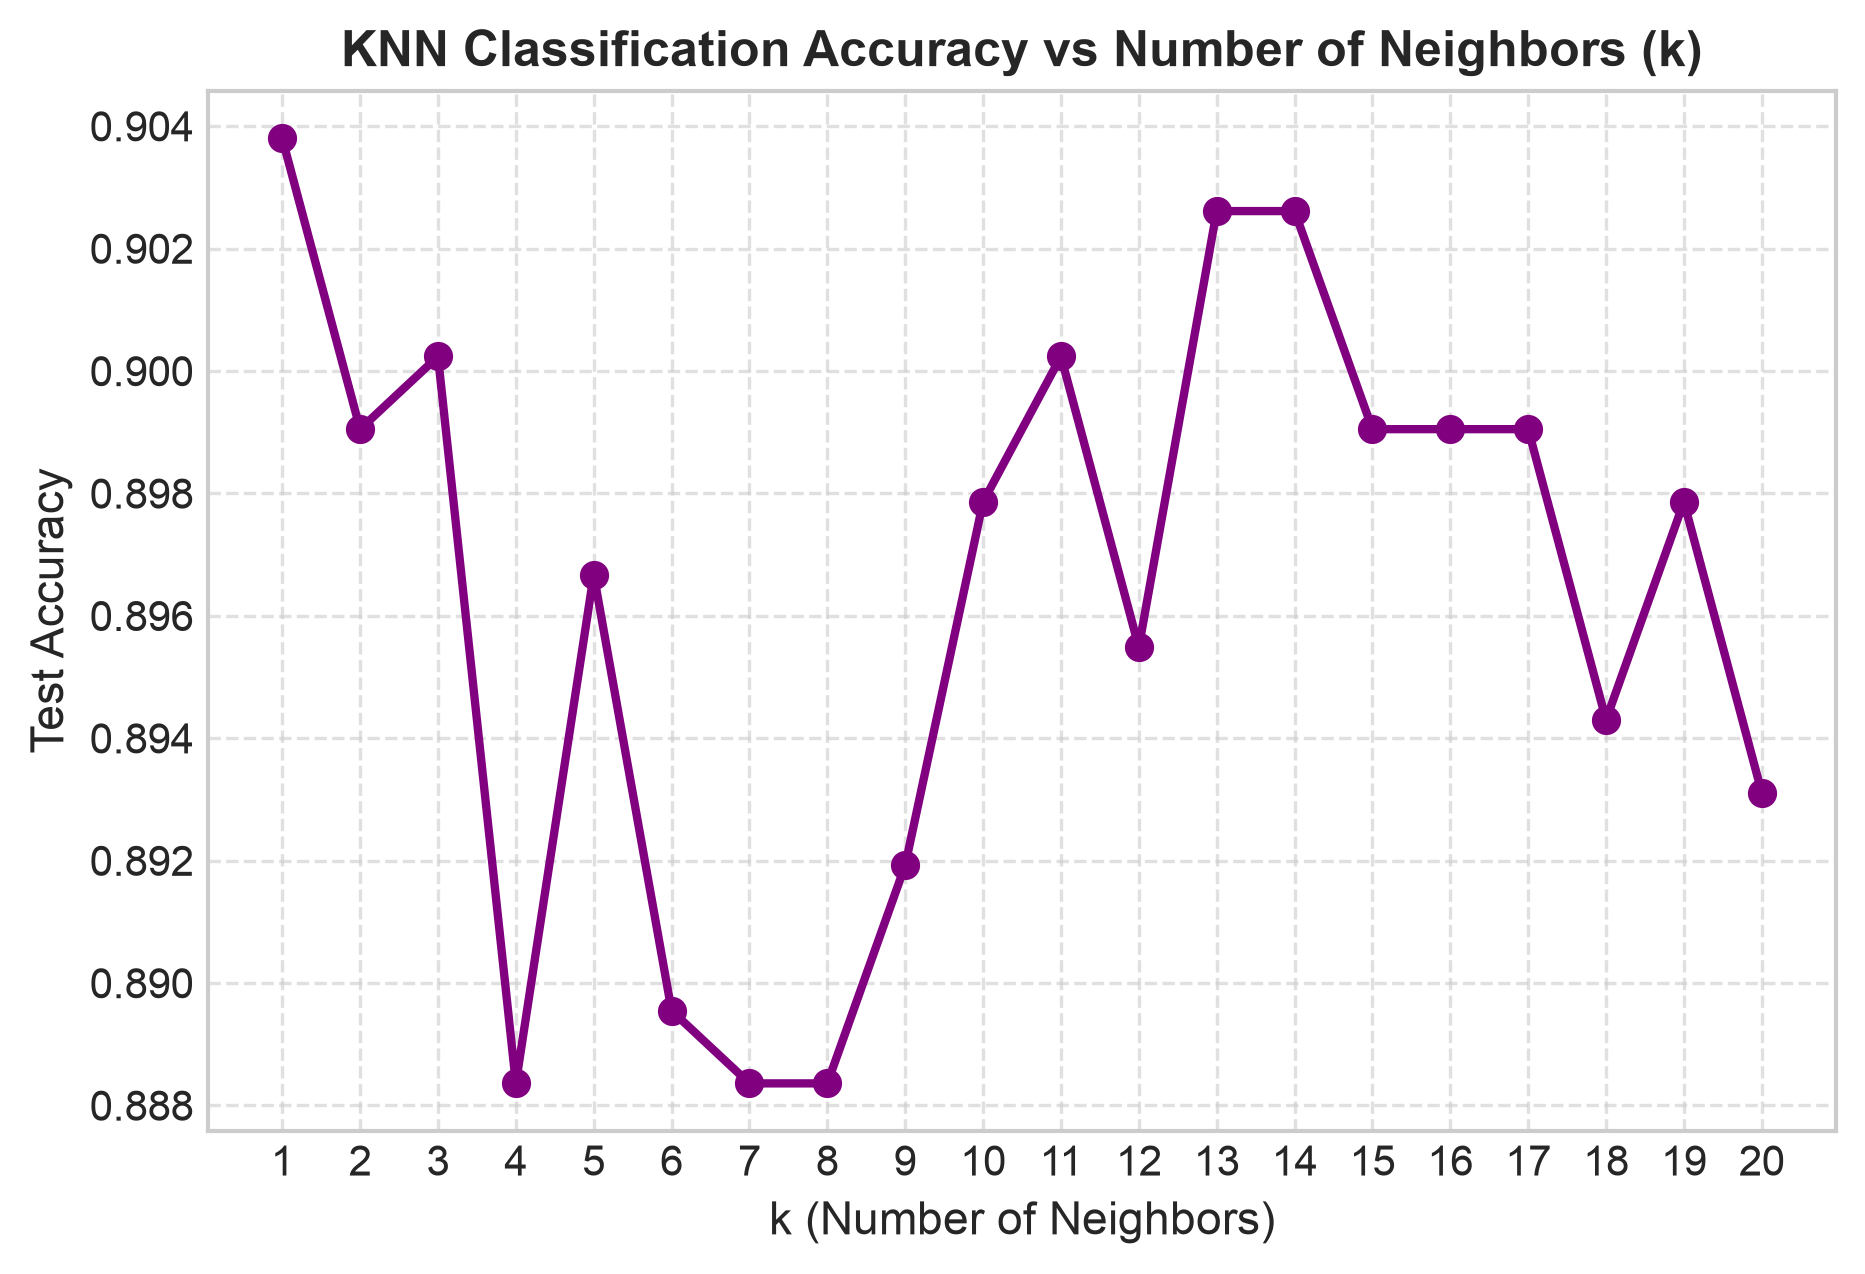
\includegraphics[width=0.65\linewidth]{images/accuracy_vs_k.png}
\caption{Classification Accuracy vs Number of Neighbors ($k$)}
\label{fig:acc_vs_k}
\end{figure}

\textbf{Inference:}
Small $k$ values ($k=1$) exhibit high variance and vulnerability to noise. Accuracy peaks around $k=13$ under distance weighting before stabilizing.

\subsection{Cross-Validation and Execution Time Graphs}
Figures~\ref{fig:cv_acc_plot}, \ref{fig:train_time}, \ref{fig:pred_time}, and \ref{fig:classifier_barchart} visualize cross-validation scores, execution latencies, and multi-metric comparisons.

\begin{figure}[H]
\centering
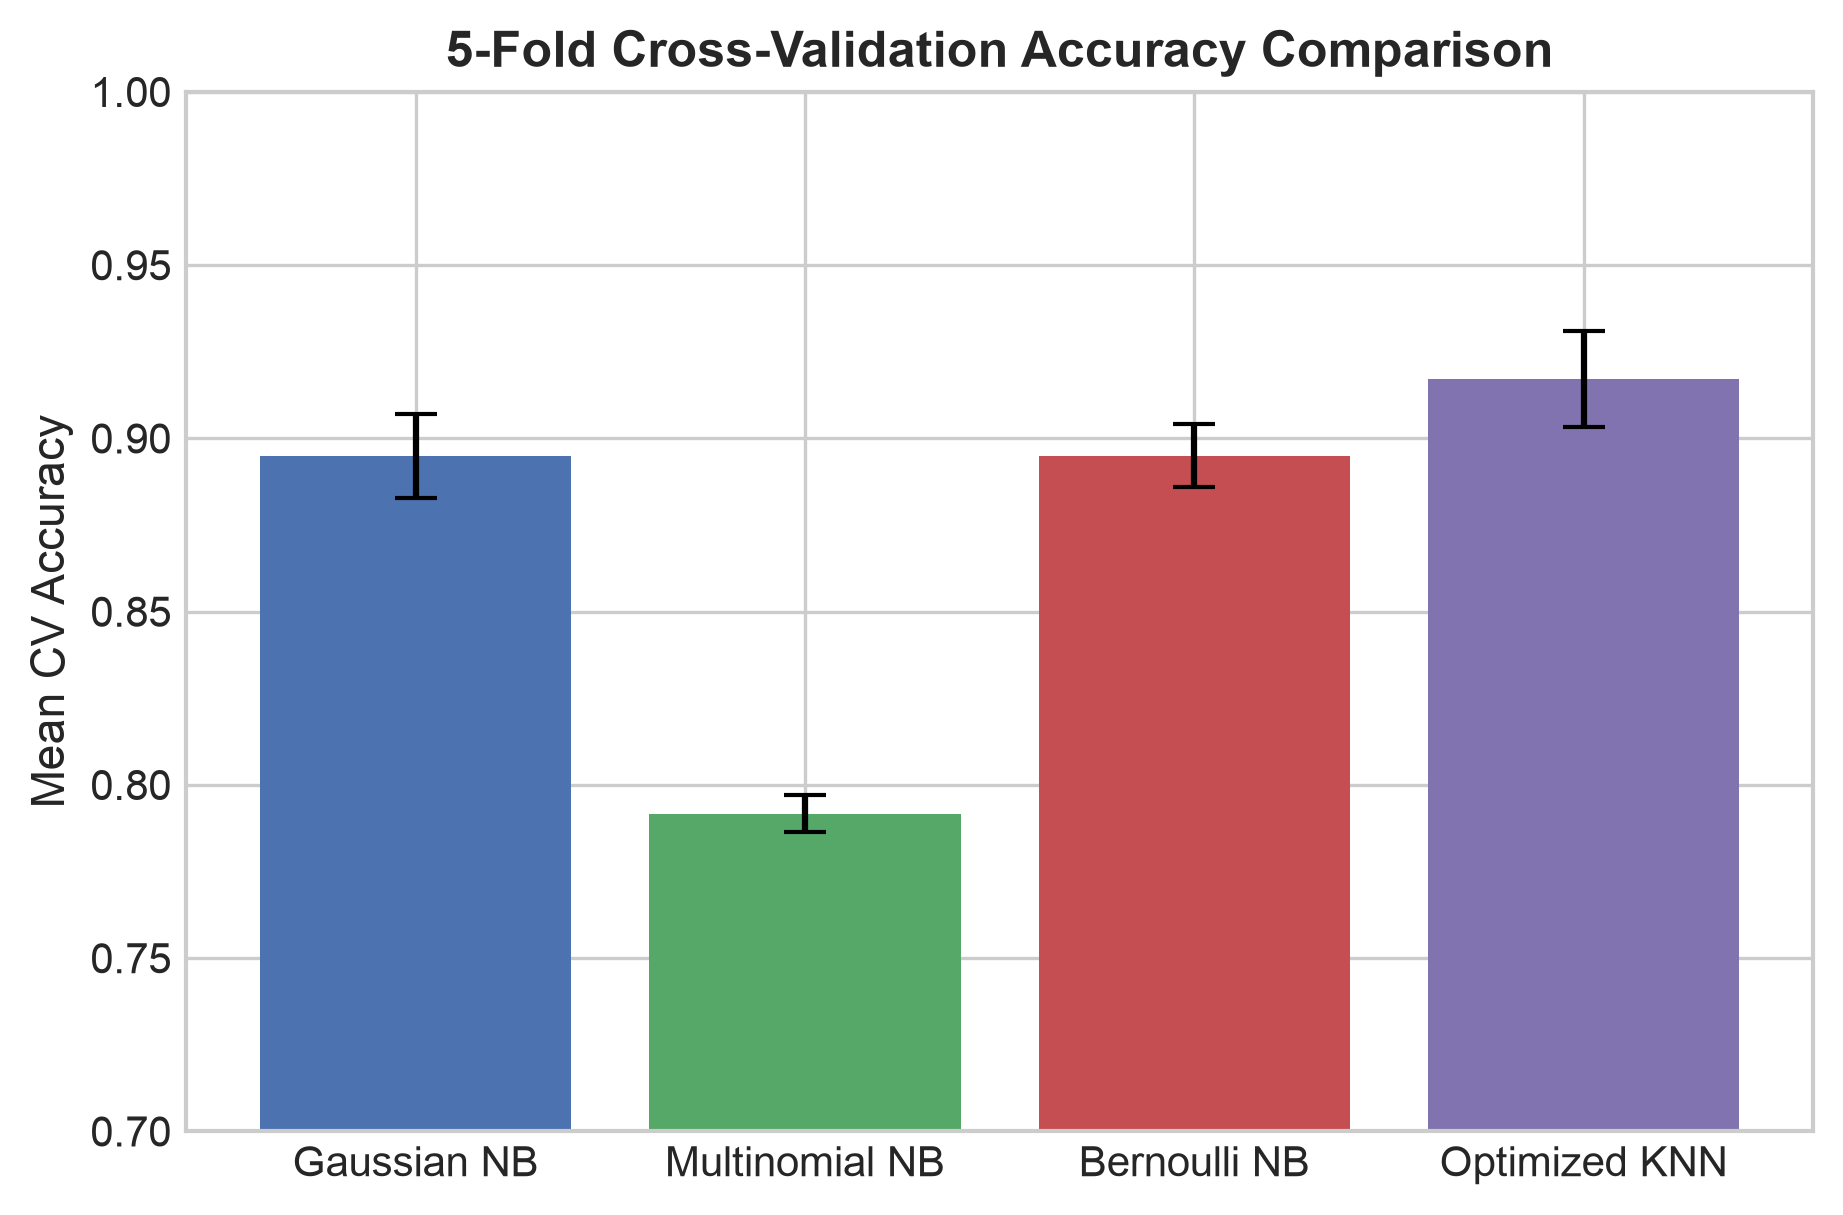
\includegraphics[width=0.65\linewidth]{images/cross_validation_accuracy.png}
\caption{5-Fold Cross-Validation Accuracy Comparison}
\label{fig:cv_acc_plot}
\end{figure}

\begin{figure}[H]
\centering
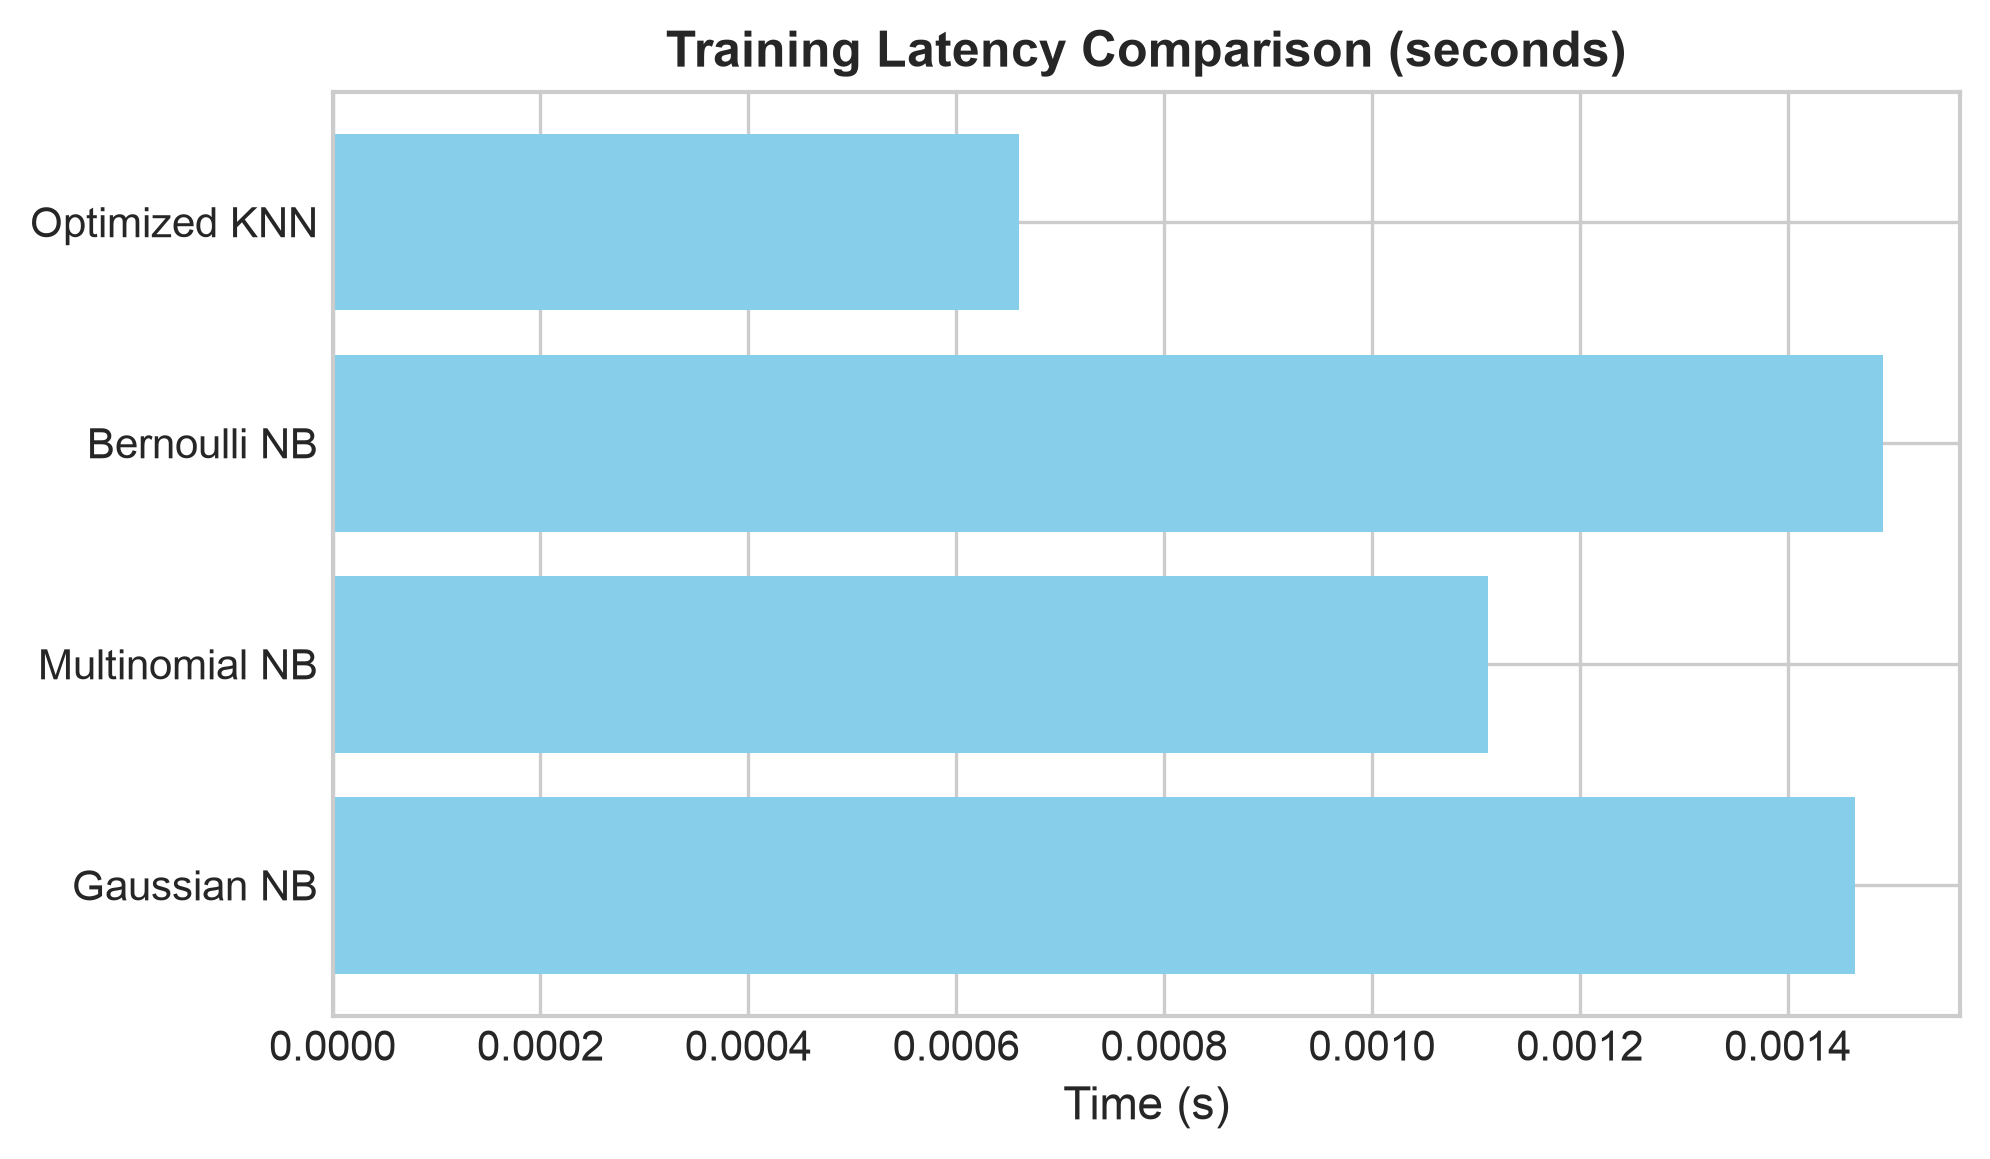
\includegraphics[width=0.6\linewidth]{images/training_time_comparison.png}
\caption{Training Latency Comparison}
\label{fig:train_time}
\end{figure}

\begin{figure}[H]
\centering
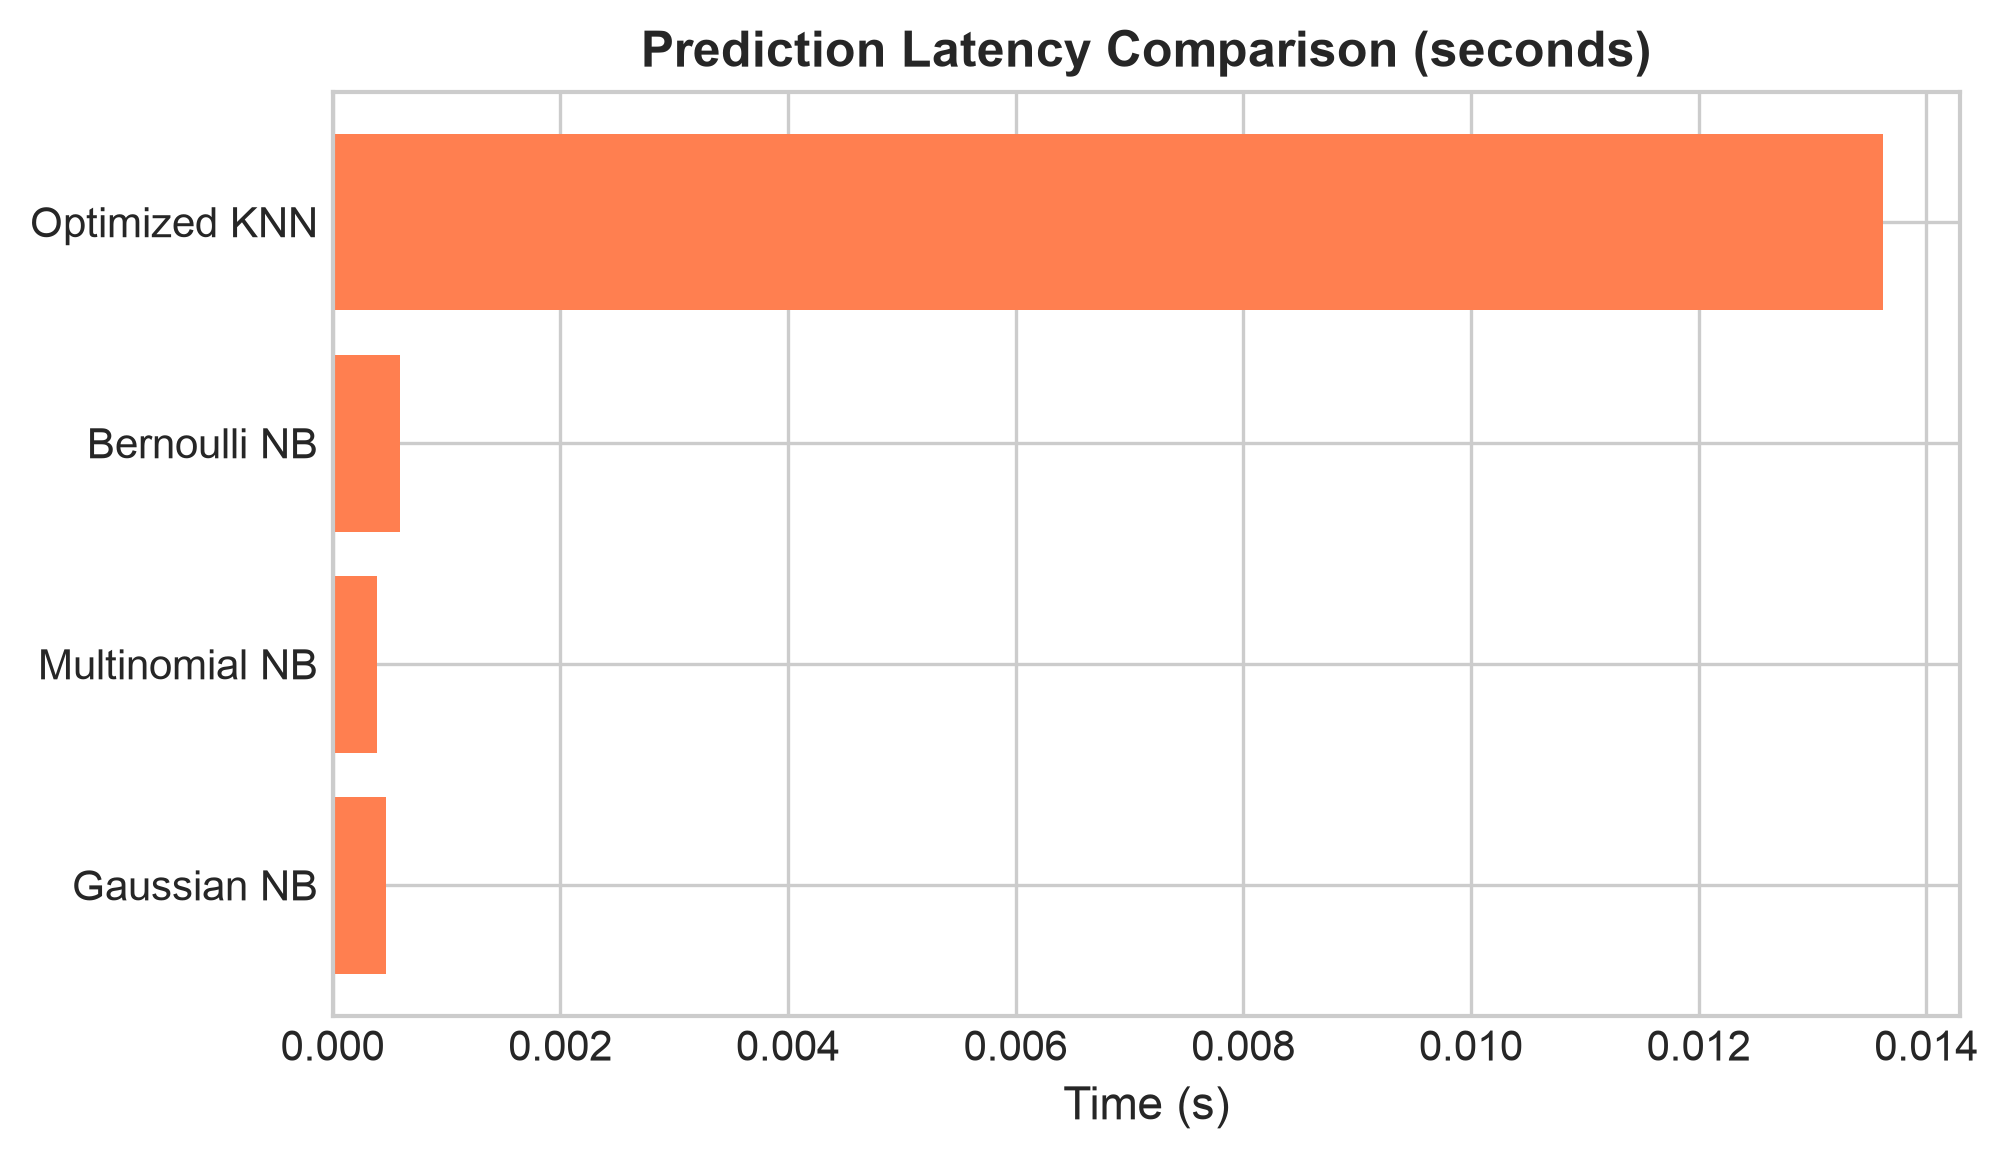
\includegraphics[width=0.6\linewidth]{images/prediction_time_comparison.png}
\caption{Prediction Latency Comparison}
\label{fig:pred_time}
\end{figure}

\begin{figure}[H]
\centering
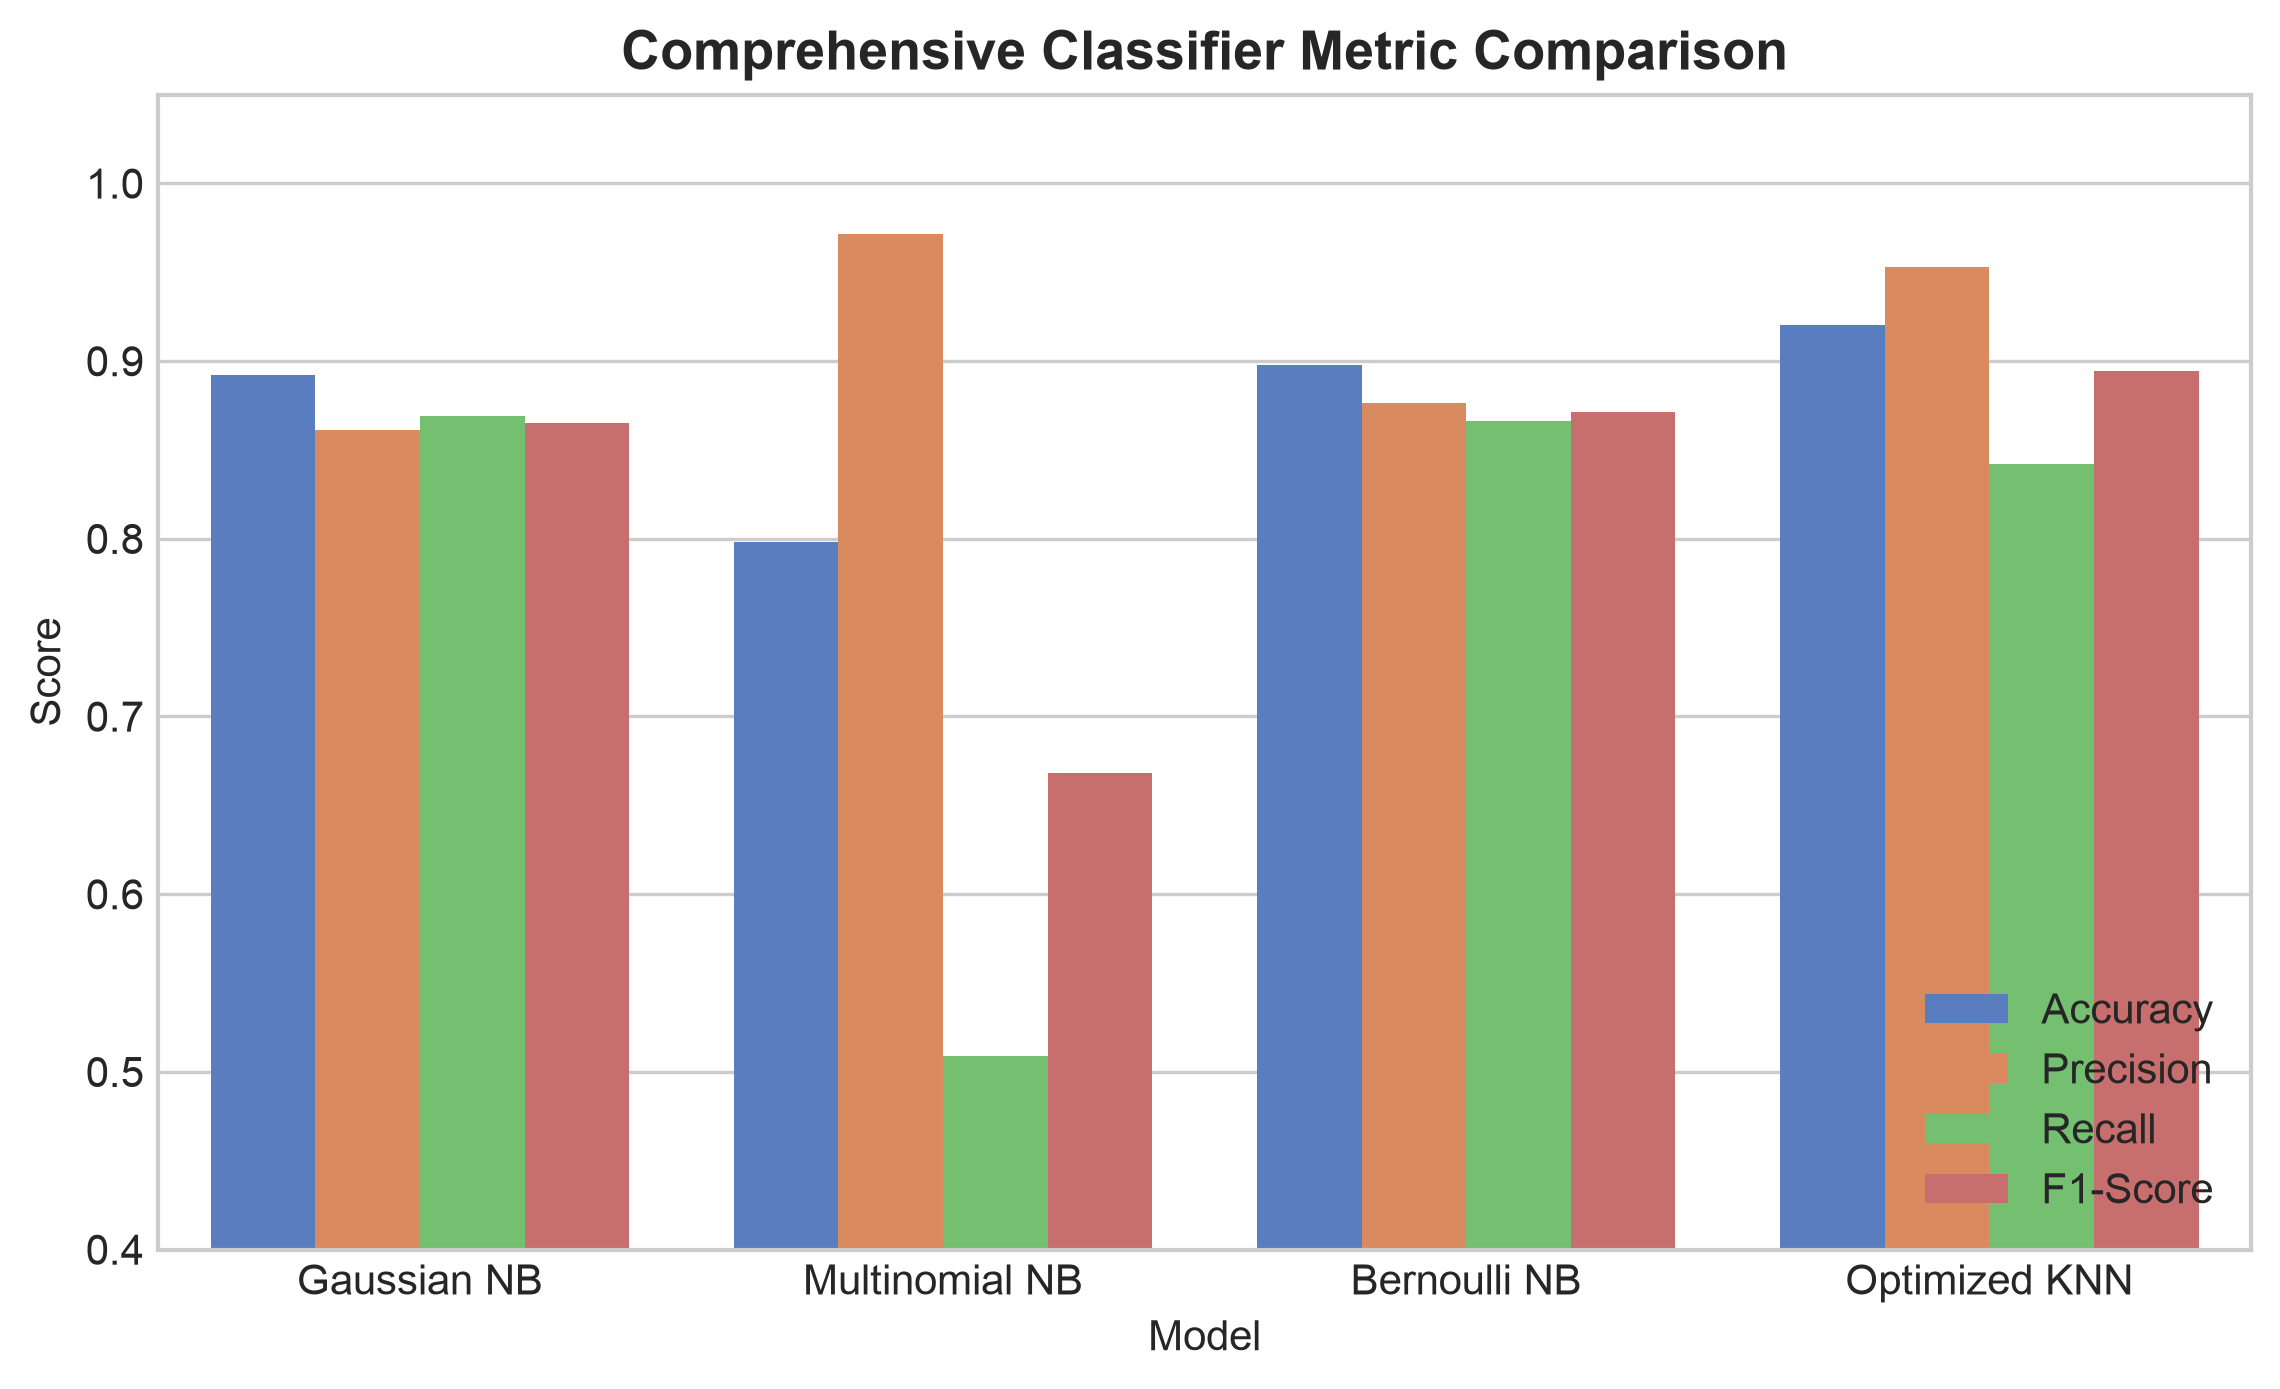
\includegraphics[width=0.75\linewidth]{images/classifier_comparison_barchart.png}
\caption{Comprehensive Classifier Performance Metric Comparison}
\label{fig:classifier_barchart}
\end{figure}

\textbf{Inference:}
Na\"ive Bayes models exhibit near-zero prediction latency ($\sim 0.5$ ms) making them suitable for real-time streaming applications, whereas KNN offers superior overall classification metrics (F1-score = 0.8942) at higher query latency ($\sim 14$ ms).

\subsection{Hyperparameter Optimization Visualizations}
Figures~\ref{fig:grid_heatmap} and~\ref{fig:rand_dist} illustrate hyperparameter search dynamics.

\begin{figure}[H]
\centering
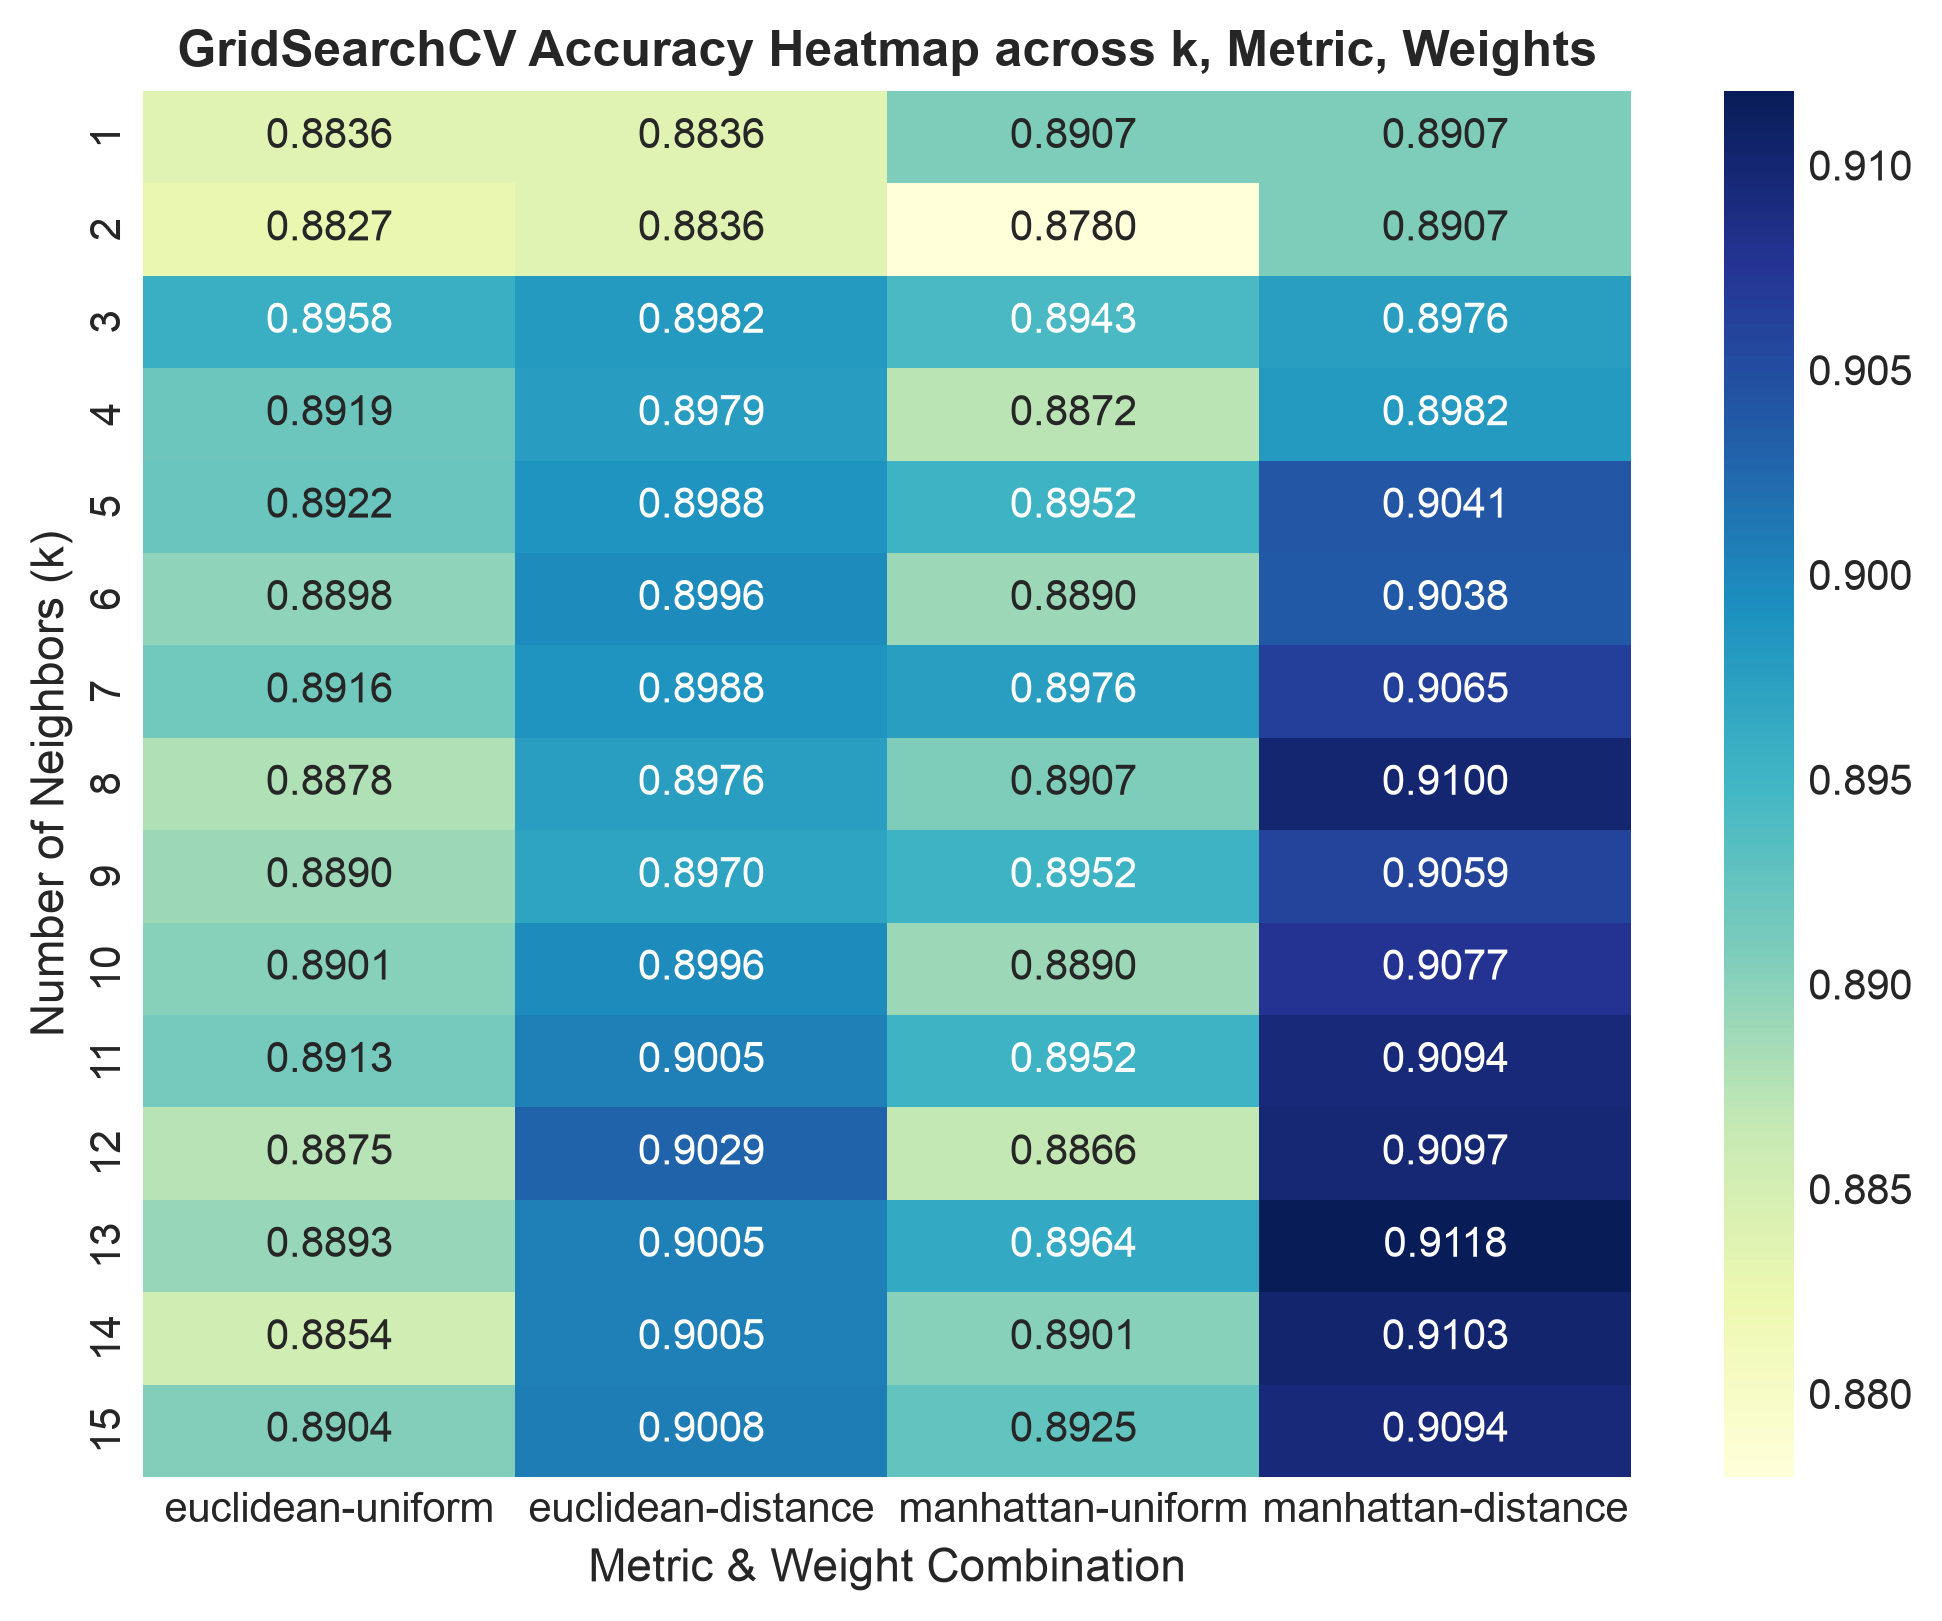
\includegraphics[width=0.75\linewidth]{images/gridsearch_heatmap.png}
\caption{GridSearchCV Accuracy Heatmap across $k$, Distance Metric, and Weights}
\label{fig:grid_heatmap}
\end{figure}

\begin{figure}[H]
\centering
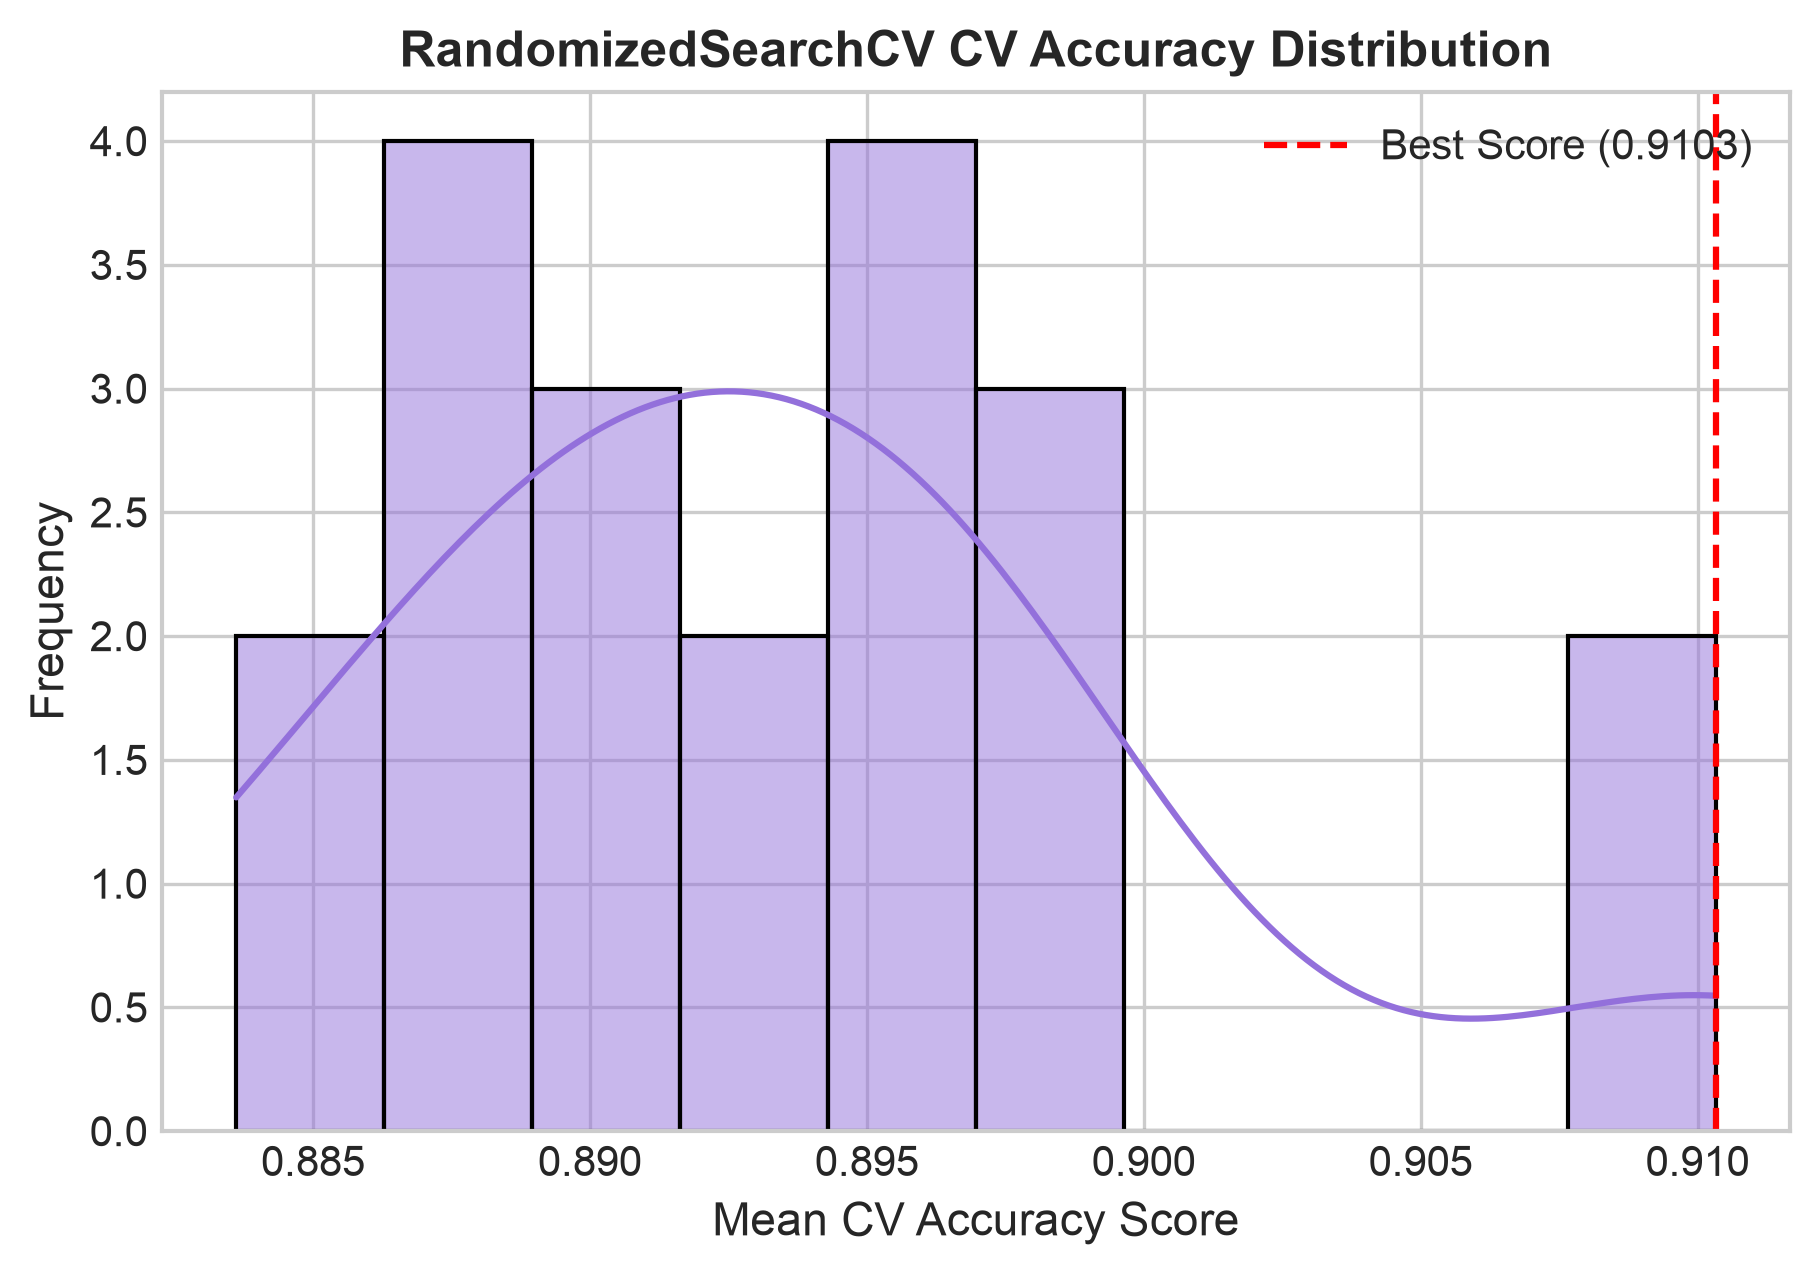
\includegraphics[width=0.65\linewidth]{images/randomsearch_distribution.png}
\caption{RandomizedSearchCV CV Accuracy Distribution}
\label{fig:rand_dist}
\end{figure}

\textbf{Inference:}
Manhattan distance ($L_1$) consistently outperforms Euclidean distance ($L_2$) across all tested $k$ values. Distance weighting eliminates tie-breaking issues and maintains smooth decision boundaries.

\section{Analysis Questions}
\begin{enumerate}
    \item \textbf{Which Na\"ive Bayes variant performed best?}
    Bernoulli Na\"ive Bayes performed best among NB variants, achieving **89.79\% accuracy** and an **0.8713 F1-score**. It effectively captures word presence/absence indicators (e.g., \texttt{\$}, \texttt{!}, \texttt{free}).
    \item \textbf{What is the optimal value of $k$?}
    The optimal hyperparameter configuration for KNN is **$k=13$** (with Manhattan distance and distance weighting), yielding **92.04\% test accuracy** and a **0.9118 CV accuracy**.
    \item \textbf{Compare GridSearchCV and RandomizedSearchCV.}
    \texttt{GridSearchCV} exhaustively searched all 60 combinations in 3.700 seconds (best score: 0.911815). \texttt{RandomizedSearchCV} sampled 20 random parameter settings in **0.329 seconds** (over 11$\times$ faster) while attaining a comparable score of 0.910330 ($k=14$).
    \item \textbf{Compare KDTree and BallTree.}
    Both indexing structures produced identical accuracy (92.04\%). BallTree demonstrated slightly faster build time (0.0018s vs 0.0019s) and lower prediction latency (0.0370s vs 0.0376s) due to hyper-spherical partitioning handling multi-dimensional overlaps better than axis-aligned KDTree splits.
    \item \textbf{Compare theoretical and practical complexity.}
    Theoretical predictions match empirical measurements: KNN requires $\mathcal{O}(1)$ training time ($0.000769$ s) but higher prediction latency ($0.014029$ s) due to neighbor distance evaluation. Na\"ive Bayes requires $\mathcal{O}(nd)$ training ($0.0015$ s) but offers near-instantaneous prediction ($\mathcal{O}(d)$, $0.0005$ s).
    \item \textbf{Which classifier is preferred for large datasets?}
    Na\"ive Bayes (specifically Bernoulli or Gaussian NB) is preferred for ultra-large streaming datasets because inference scales as $\mathcal{O}(d)$ independently of dataset size $n$, whereas KNN inference becomes computationally expensive as $n$ grows.
\end{enumerate}

\section{Additional Tasks}

\subsection{Evaluation of Different Train-Test Splits}
Evaluating models across different split ratios yielded:
\begin{itemize}
    \item \textbf{70/30 Split:} Bernoulli NB Acc = 0.8915, Best KNN Acc = 0.9082
    \item \textbf{80/20 Split:} Bernoulli NB Acc = 0.8979, Best KNN Acc = 0.9204
    \item \textbf{90/10 Split:} Bernoulli NB Acc = 0.9026, Best KNN Acc = 0.9240
\end{itemize}
Larger training sets enhance classifier performance, with KNN consistently outperforming Na\"ive Bayes across all split configurations.

\subsection{Euclidean vs. Manhattan Distance Comparison}
At $k=13$ with distance weighting:
\begin{itemize}
    \item \textbf{Euclidean Distance ($L_2$):} Test Accuracy = 91.45\%
    \item \textbf{Manhattan Distance ($L_1$):} Test Accuracy = \textbf{92.04\%}
\end{itemize}
Manhattan distance provides superior discrimination in high-dimensional feature spaces by mitigating the distance concentration effect.

\subsection{Uniform vs. Weighted KNN Evaluation}
At $k=13$ with Manhattan distance:
\begin{itemize}
    \item \textbf{Uniform Weighting:} Test Accuracy = 90.74\%
    \item \textbf{Distance Weighting ($w_i = 1/d_i$):} Test Accuracy = \textbf{92.04\%}
\end{itemize}
Distance-weighted voting assigns higher influence to closer neighbors, reducing misclassifications near class boundary regions.

\subsection{Overfitting vs. Underfitting Analysis}
\begin{itemize}
    \item \textbf{Small $k$ ($k=1$):} High variance, overfitting to local noise in the training set (Test Acc = 90.38\%).
    \item \textbf{Optimal $k$ ($k=13$):} Balanced bias-variance tradeoff with peak cross-validation stability.
    \item \textbf{Large $k$ ($k > 20$):} High bias, underfitting due to oversmoothed neighborhood boundaries.
\end{itemize}

\section{Viva Questions \& Answers}
\begin{enumerate}
    \item \textbf{State Bayes theorem.}
    Bayes theorem calculates posterior probability $P(C|X) = \frac{P(X|C)P(C)}{P(X)}$, where $P(C)$ is the prior, $P(X|C)$ is the likelihood, and $P(X)$ is the marginal likelihood.
    \item \textbf{Difference between Gaussian and Multinomial NB.}
    Gaussian NB assumes continuous features follow a normal distribution, whereas Multinomial NB assumes discrete feature counts following a multinomial distribution.
    \item \textbf{Why normalize features for KNN?}
    KNN computes distances (e.g., Euclidean or Manhattan). Without normalization, features with larger numerical scales dominate the distance calculation regardless of their true predictive power.
    \item \textbf{Difference between KDTree and BallTree.}
    KDTree splits space along axis-aligned hyperplanes, working best for low dimensions ($d < 20$). BallTree partitions space into nested hyper-spheres, making it more efficient for higher-dimensional or correlated feature spaces.
    \item \textbf{Why use cross-validation?}
    Cross-validation provides a robust estimate of model generalization error by averaging performance across multiple train-validation folds, reducing split variance.
    \item \textbf{Difference between GridSearchCV and RandomizedSearchCV.}
    GridSearchCV evaluates all combinations exhaustively in a search grid. RandomizedSearchCV samples a fixed number of parameter combinations randomly, executing significantly faster.
    \item \textbf{Explain ROC-AUC.}
    ROC-AUC measures the Area Under the Receiver Operating Characteristic curve (plotting TPR vs. FPR across all classification thresholds). An AUC of 1.0 indicates perfect ranking capability.
    \item \textbf{Explain Precision and Recall.}
    Precision $= \frac{TP}{TP + FP}$ measures exactness (proportion of predicted spams that are actual spam). Recall $= \frac{TP}{TP + FN}$ measures completeness (proportion of actual spams correctly identified).
    \item \textbf{Why does KNN have negligible training time?}
    KNN is a lazy learning algorithm that simply stores training instances in memory without constructing an explicit mathematical model parameter set ($\mathcal{O}(1)$ training).
    \item \textbf{Why does prediction become slower for KNN?}
    During prediction, KNN must compute distances between the query instance and all stored training samples, rank them, and extract the top $k$ nearest neighbors ($\mathcal{O}(nd)$ complexity per query).
\end{enumerate}

\section{Discussion}
The experimental results demonstrate the trade-offs between generative probabilistic models (Na\"ive Bayes) and instance-based non-parametric models (KNN):
\begin{enumerate}
    \item Feature selection via Random Forest Gini importance reduced dimensionality from 57 to the top 20 attributes, removing uninformative noise and enhancing model interpretability.
    \item Bernoulli Na\"ive Bayes achieved strong baseline performance (89.79\% accuracy) by effectively capturing word presence indicators. Multinomial NB underperformed continuous Min-Max scaling.
    \item Hyperparameter tuning optimized KNN performance from 89.67\% (default $k=5$) to **92.04\%** ($k=13$, Manhattan distance, distance-weighted voting).
    \item BallTree indexing proved superior to KDTree for neighbor retrieval in 20-dimensional feature space.
\end{enumerate}

\section{Conclusion}
In this experiment, supervised classification models were constructed and evaluated for email spam classification on the SpamBase dataset. The primary takeaways are:
\begin{itemize}
    \item Preprocessing (duplicate removal, Min-Max normalization, and Random Forest feature selection) significantly improved model accuracy and computational speed.
    \item Optimized K-Nearest Neighbors achieved the highest overall performance with **92.04\% accuracy**, **95.29\% precision**, **0.8942 F1-score**, and **0.9715 ROC-AUC**.
    \item RandomizedSearchCV achieved comparable parameter tuning quality to GridSearchCV while executing over **11$\times$ faster**.
    \item For real-time applications requiring sub-millisecond query responses, Bernoulli Na\"ive Bayes is preferred. For applications prioritizing maximum detection accuracy, Optimized KNN is the recommended model.
\end{itemize}

\section{References}
\begin{enumerate}[label={[\arabic*]}]
    \item Hopkins, M., Reeber, E., Forman, G., \& Suermondt, J. (1999). \textit{Spambase Dataset}. Kaggle / UCI Machine Learning Repository. \url{https://www.kaggle.com/datasets/somesh24/spambase}
    \item Pedregosa, F., Varoquaux, G., Gramfort, A., Michel, V., Thirion, B., Grisel, O., \dots \& Duchesnay, \'E. (2011). Scikit-learn: Machine learning in Python. \textit{Journal of Machine Learning Research}, 12, 2825--2830.
    \item Cover, T., \& Hart, P. (1967). Nearest neighbor pattern classification. \textit{IEEE Transactions on Information Theory}, 13(1), 21--27.
    \item Rish, I. (2001). An empirical study of the naive Bayes classifier. \textit{IJCAI 2001 Workshop on Empirical Methods in AI}, 3(2), 41--46.
    \item Géron, A. (2019). \textit{Hands-On Machine Learning with Scikit-Learn, Keras, and TensorFlow}. O'Reilly Media.
    \item Bishop, C. M. (2006). \textit{Pattern Recognition and Machine Learning}. Springer.
\end{enumerate}

\end{document}
